% Untangling Federal Jurisdiction
% Part 3

% All content comes from Stephen Pratt. I have no idea if he approves of this effort or not.

\documentclass{beamer}
\usetheme{Madrid}
%\usetheme{Goettingen}
\usefonttheme{serif}
\usefonttheme{structuresmallcapsserif}
% \usepackage[font=small,labelfont=bf]{caption}
\usepackage{xcolor}
\usepackage{rotating}

\setbeamerfont{section title}{parent=title}
\setbeamercolor{section title}{parent=titlelike}
\defbeamertemplate*{section page}{default}[1][]
{
    \centering
    \begin{beamercolorbox}[sep=8pt,center,#1]{section title}
        \usebeamerfont{section title}\insertsection\par
    \end{beamercolorbox}
}
\newcommand*{\sectionpage}{\usebeamertemplate*{section page}}

\def\Put(#1,#2)#3{\leavevmode\makebox(0,0){\put(#1,#2){#3}}}

\makeatletter
\setbeamertemplate{footline}
{
    % Commented out to remove footer line entirely
%    \leavevmode%
%    \hbox{%
%    \begin{beamercolorbox}[wd=.333333\paperwidth,ht=2.25ex,dp=1ex,center]{author in head/foot}%
%        \usebeamerfont{author in head/foot}\insertshortauthor%~~\beamer@ifempty{\insertshortinstitute}{}{(\insertshortinstitute)}
%    \end{beamercolorbox}%
%    \begin{beamercolorbox}[wd=.333333\paperwidth,ht=2.25ex,dp=1ex,center]{title in head/foot}%
%        \usebeamerfont{title in head/foot}\insertshorttitle
%    \end{beamercolorbox}%
%    \begin{beamercolorbox}[wd=.333333\paperwidth,ht=2.25ex,dp=1ex,right]{date in head/foot}%
%        \usebeamerfont{date in head/foot}\insertshortdate{}\hspace*{2em}
%        \insertframenumber{} / \inserttotalframenumber\hspace*{2ex} 
%    \end{beamercolorbox}}%
%    \vskip0pt%
}
\makeatother

\newenvironment<>{varblock}[2][\textwidth]{
    \begin{center}
        \begin{minipage}{#1}
            \setlength{\textwidth}{#1}
            \begin{actionenv}#3
                \def\insertblocktitle{#2}
                \par
                \usebeamertemplate{block begin}}
            {\par
                \usebeamertemplate{block end}
            \end{actionenv}
        \end{minipage}
    \end{center}
}

\DeclareGraphicsExtensions{.pdf,.png,.jpg}


\begin{document}
\unitlength=1pt

%\section{Life after Kleppe}
%\frame{\sectionpage}
%
%\begin{frame}{Gouvernor Morris and the Property Clause}
%    \centering
%    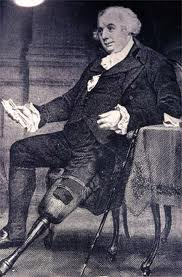
\includegraphics[height=.8\textheight]{img/morris-full.png} \\
%\end{frame}
%
%\begin{frame}
%    \begin{columns}[onlytextwidth]
%        \column{0.5\textwidth}
%            \textbf{Letter, December 4, 1803} \\
%            Morris, by his own admission, had attempted to concoct a deception,
%            if not a fraud, hidden in duplicitous wording of the Property
%            Clause.
%
%        \column{0.5\textwidth}
%            \centering
%            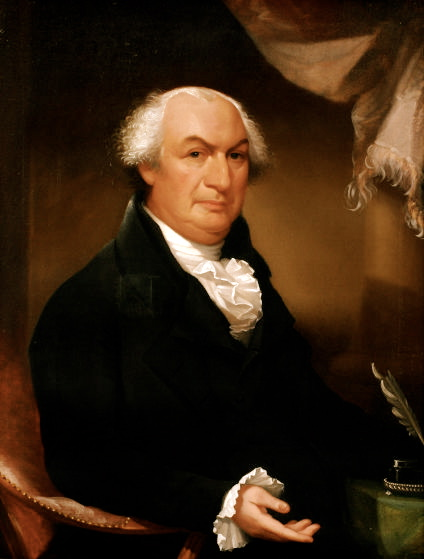
\includegraphics[width=0.95\textwidth]{img/morris-portrait.png} \\
%            Gouvernor Morris, 1803 \\
%    \end{columns}
%\end{frame}
%
%\begin{frame}
%    \begin{columns}[onlytextwidth]
%        \column{0.5\textwidth}
%            \textbf{Letter, December 4, 1803} \\
%            ``I went as far as circumstances would permit\ldots Had it been
%            more pointedly expressed, a strong opposition would have been made.''
%
%        \column{0.5\textwidth}
%            \centering
%            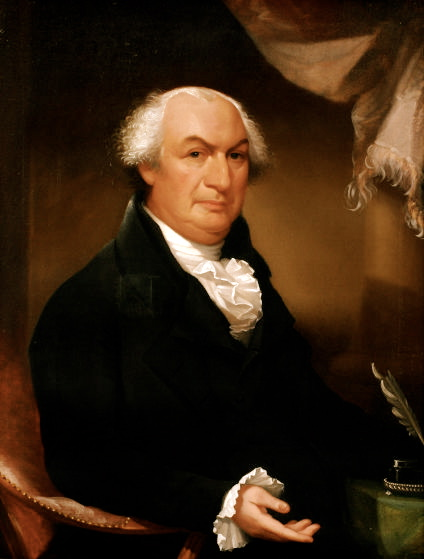
\includegraphics[width=0.95\textwidth]{img/morris-portrait.png} \\
%            Gouvernor Morris, 1803 \\
%    \end{columns}
%\end{frame}
%
%\begin{frame}{1976, Property Clause Revisited}
%    \centering
%    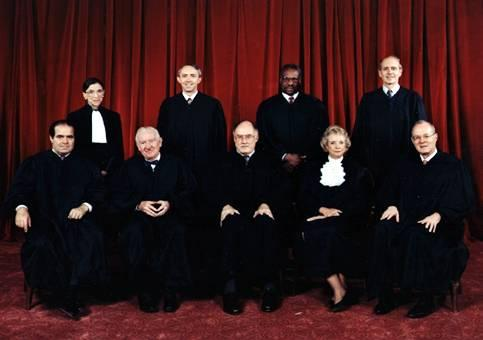
\includegraphics[width=0.75\textwidth]{img/sc-1976.png} \\
%\end{frame}
%
%\begin{frame}
%    \begin{columns}[onlytextwidth]
%        \column{0.5\textwidth}
%            \centering
%            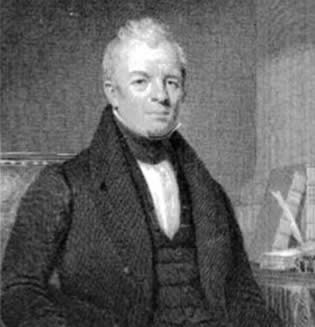
\includegraphics[width=0.95\textwidth]{img/james-kent.png} \\
%            James Kent, 1826 \\
%            \emph{Commentaries on American Law}, 4 vols. \\
%
%        \column{0.5\textwidth}
%            { \large ``[Judges] roam at large in the trackless field of their own imaginations.''}
%    \end{columns}
%\end{frame}
%
%\begin{frame}{1976, Property Clause Revisited}
%    \centering
%    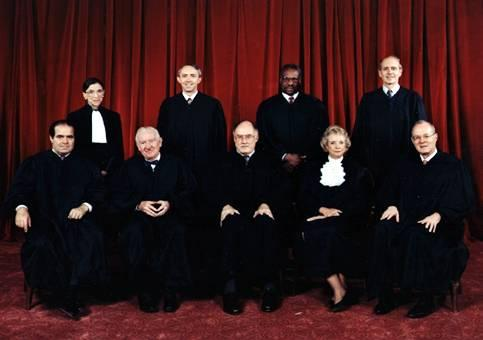
\includegraphics[width=0.75\textwidth]{img/sc-1976.png} \\
%    ``\ldots make all needful rules and regulations\ldots'' \\
%    \Put(260,60){
\includegraphics[width=.2\textwidth]{img/sherlock.png}}
%\end{frame}
%
%\begin{frame}{``Emanations from Penumbrae''}
%   \centering
%   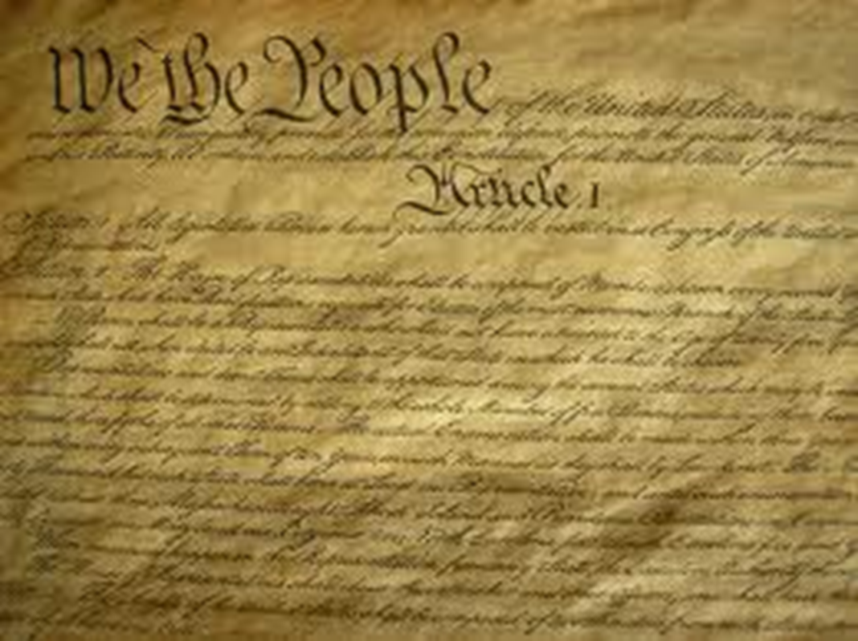
\includegraphics[height=.7\textheight]{img/constitution.png} \\
%   \Put(200,080){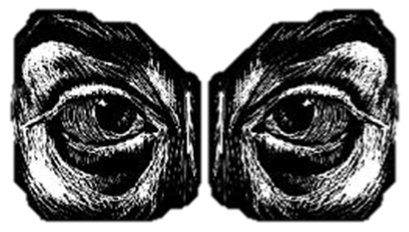
\includegraphics[width=.4\textwidth]{img/eyes.png}}
%\end{frame}
%
%\begin{frame}{``Emanations from Penumbrae''}
%   \centering
%   
\includegraphics[height=.7\textheight]{img/fire.png} \\
%   \Put(200,080){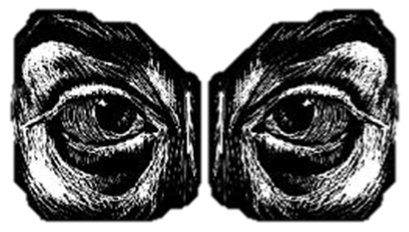
\includegraphics[width=.4\textwidth]{img/eyes.png}}
%\end{frame}
%
%\begin{frame}{Kleppe v. New Mexico, 1976}
%    \centering
%    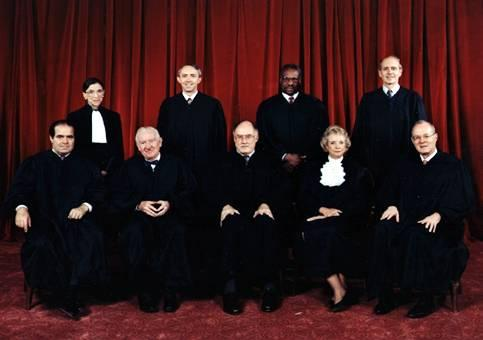
\includegraphics[width=0.75\textwidth]{img/sc-1976.png} \\
%    { \large Federal legislative power over public lands is ``complete'' and
%    ``without limitation.'' \\ }
%    \Put(260,160){
\includegraphics[width=.2\textwidth]{img/sherlock.png}}
%\end{frame}
%
%\begin{frame}
%    \begin{columns}[onlytextwidth]
%        \column{0.5\textwidth}
%            { \large Imagine Gouvernor Morris now\ldots }
%        \column{0.5\textwidth}
%            \centering
%            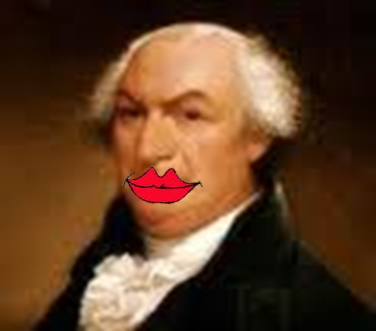
\includegraphics[width=0.95\textwidth]{img/morris-smile.png} \\
%    \end{columns}
%\end{frame}
%
%\begin{frame}{Jurisdiction Clause Family --- Supremacy}
%    \centering
%    
\includegraphics[height=0.85\textheight]{img/family.png} \\
%    \huge{\textbf{ \color{white}
%        %\Put(25, 300){\begin{sideways}\colorbox{blue}{Admissions}\end{sideways}}
%        %\Put(60, 300){\begin{sideways}\colorbox{blue}{Claims}\end{sideways}}
%        %\Put(90, 300){\begin{sideways}\colorbox{blue}{Property}\end{sideways}}
%        %\Put(134, 300){\begin{sideways}\colorbox{blue}{Guarantee}\end{sideways}}
%        %\Put(168, 300){\begin{sideways}\colorbox{blue}{Enclave}\end{sideways}}
%        %\Put(200, 300){\begin{sideways}\colorbox{blue}{Engagements}\end{sideways}}
%        \Put(235, 300){\begin{sideways}\colorbox{blue}{Supremacy}\end{sideways}}
%    }}
%\end{frame}
%
%\begin{frame}{Supremacy Clause}
%   \centering
%   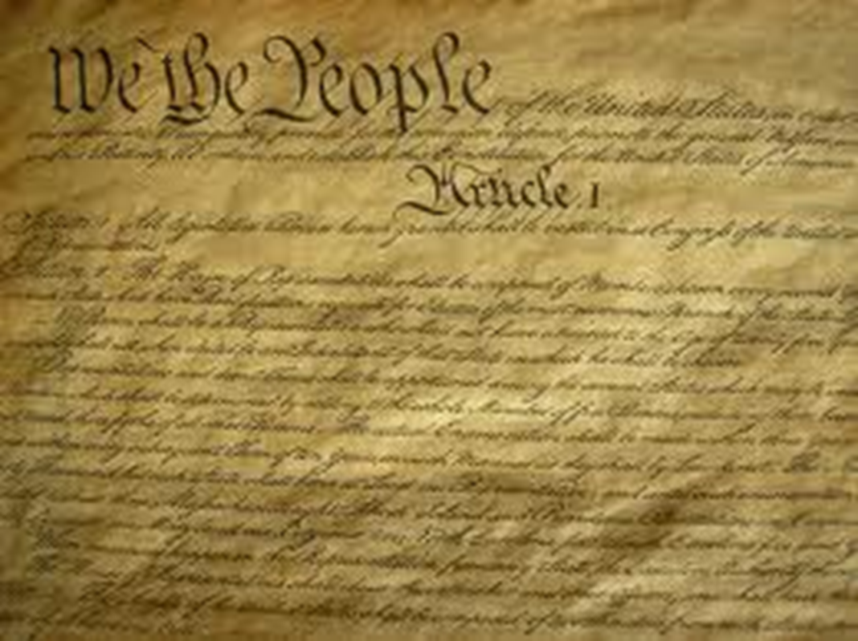
\includegraphics[height=.7\textheight]{img/constitution.png} \\
%   \textbf{Article VI, clause 2:} ``This Constitution, and the Laws of the
%   United States \emph{which shall be made in Pursuance thereof}\ldots shall be
%   the supreme Law of the Land.''
%\end{frame}
%
%\begin{frame}{United States Senate and House of Representatives}
%    \centering
%    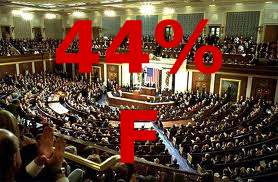
\includegraphics[width=0.75\textwidth]{img/house-senate-fail.png} \\
%\end{frame}
%
%\begin{frame}{Kleppe v. New Mexico, 1976}
%    \centering
%    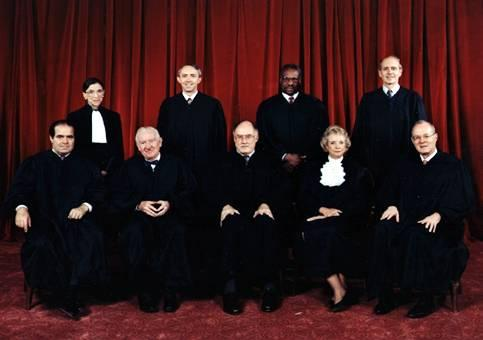
\includegraphics[width=0.65\textwidth]{img/sc-1976.png} \\
%    Congress may enact legislation governing federal lands pursuant to the
%    property clause and ``when Congress so acts, federal legislation
%    necessarily overrides conflicting state laws under the \emph{supremacy
%    clause}.''
%\end{frame}
%
%\begin{frame}{Continuum of \textbf{\emph{Sliding}} Judicial Opinions}
%    \Put(20,20){\Large \begin{turn}{50} Johnson v. McIntosh, 1823 \end{turn}}
%    \Put(50,10){\Large \begin{turn}{50} Benner v. Porter, 1850 \end{turn}}
%    \Put(80,30){\Large \begin{turn}{50} Kohl v. United States, 1875 \end{turn}}
%    \Put(110,45){\Large \begin{turn}{50} Ft. Leavenworth v. Lowe, 1885 \end{turn}}
%    \Put(130,40){\Large \begin{turn}{50} Collins v. Yosemite Park, 1938 \end{turn}}
%    \Put(170,30){\Large \begin{turn}{50} Kleppe v. New Mexico, 1976 \end{turn}}
%    \Put(190,-115){\Large \begin{turn}{50} FPLMA, 1976 \end{turn}}
%    {
%        \color{red}
%        \thicklines
%        \Put(-20, -130){ \line(1, 0){250} }
%    }
%    \pause
%    \Put(-30,100){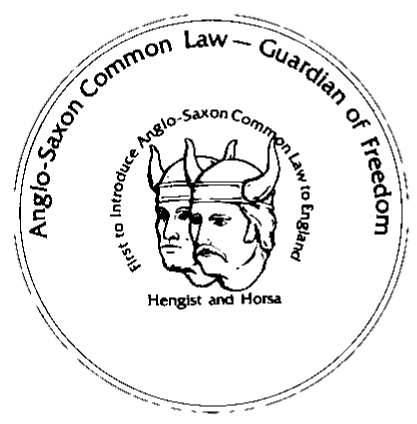
\includegraphics[width=.3\textwidth]{img/hh-coin.png}}
%    \pause
%    \Put(260,0){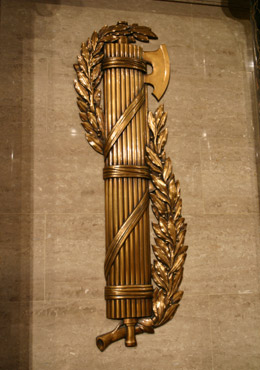
\includegraphics[height=.4\textheight]{img/fasces.png}}
%    \pause
%    \Put(30,-240){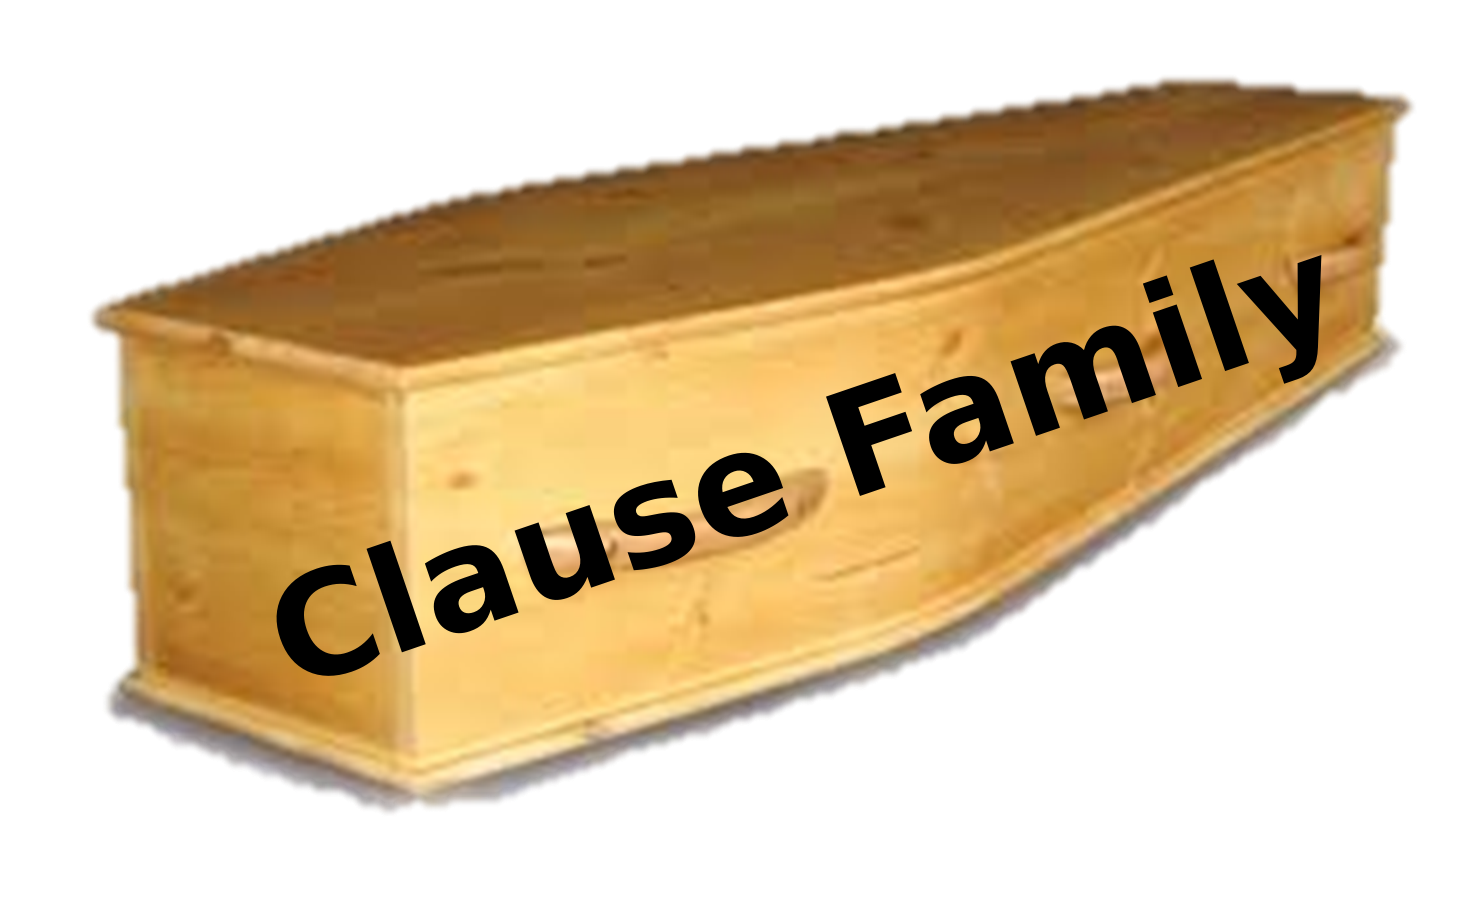
\includegraphics[width=.5\textwidth]{img/coffin-clause.png}}
%\end{frame}
%
%\begin{frame}{Here lies the Clause Family}
%    \centering
%    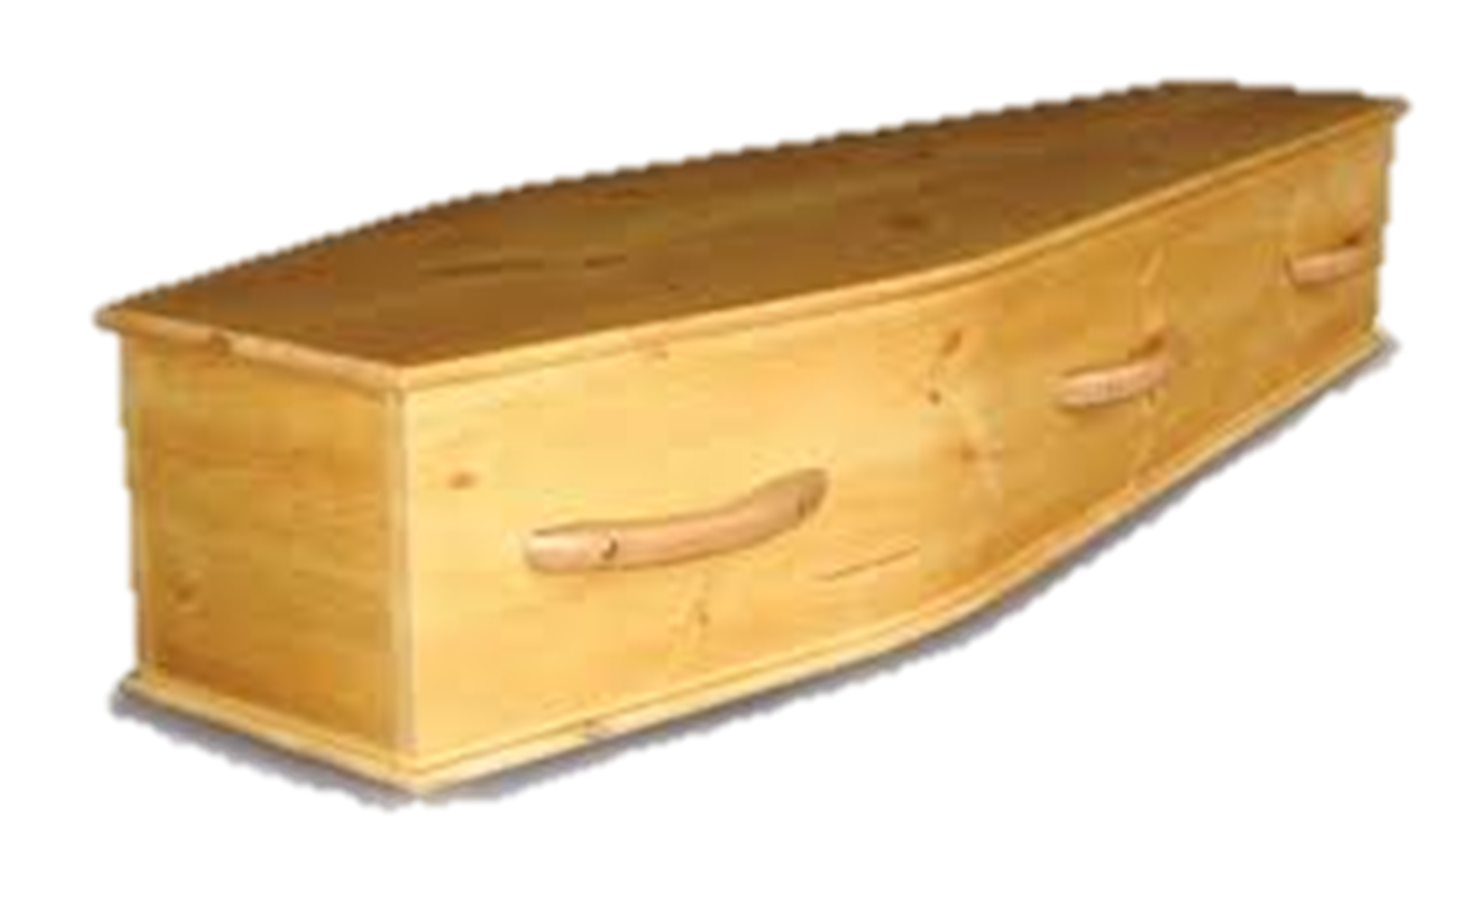
\includegraphics[width=.6\textwidth]{img/coffin.png} \\
%    { \large
%    Born March 4, 1789 \\
%    Died by Strangulation, 1976 \\
%    }
%\end{frame}
%
%\begin{frame}{126 Days after Kleppe: FLPMA}
%    \centering
%    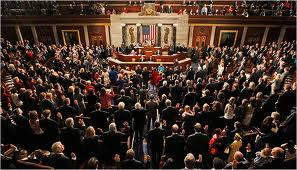
\includegraphics[width=.8\textwidth]{img/congress.png} \\
%    Federal Lands Policy and Management Act \\
%    { \large ``\ldots that it is the policy of the United States that the
%    public lands be retained in Federal ownership\ldots'' }
%\end{frame}
%
%\begin{frame}
%    
\includegraphics[width=.3\textwidth]{img/stop.png}
%    \hspace{10pt}
%    
\includegraphics[width=.3\textwidth]{img/think.png}
%    \hspace{10pt}
%    
\includegraphics[width=.3\textwidth]{img/wrong-way.png} \\
%    \vspace{20pt}
%    \begin{block}{Consequences of Kleppe}
%        Public lands within the States have been rendered jurisdictionally equivalent to pre-statehood Territories, the District of Columbia, and federal enclaves!
%    \end{block}
%\end{frame}
%
%\begin{frame}{Jurisdiction Clause Family --- Claims}
%    \centering
%    
\includegraphics[height=0.85\textheight]{img/family.png} \\
%    \huge{\textbf{ \color{white}
%        %\Put(25, 300){\begin{sideways}\colorbox{blue}{Admissions}\end{sideways}}
%        \Put(70, 300){\begin{sideways}\colorbox{blue}{Claims}\end{sideways}}
%        %\Put(90, 300){\begin{sideways}\colorbox{blue}{Property}\end{sideways}}
%        %\Put(134, 300){\begin{sideways}\colorbox{blue}{Guarantee}\end{sideways}}
%        %\Put(168, 300){\begin{sideways}\colorbox{blue}{Enclave}\end{sideways}}
%        %\Put(200, 300){\begin{sideways}\colorbox{blue}{Engagements}\end{sideways}}
%        %\Put(235, 300){\begin{sideways}\colorbox{blue}{Supremacy}\end{sideways}}
%    }}
%\end{frame}
%
%\begin{frame}{Claims Clause}
%   \centering
%   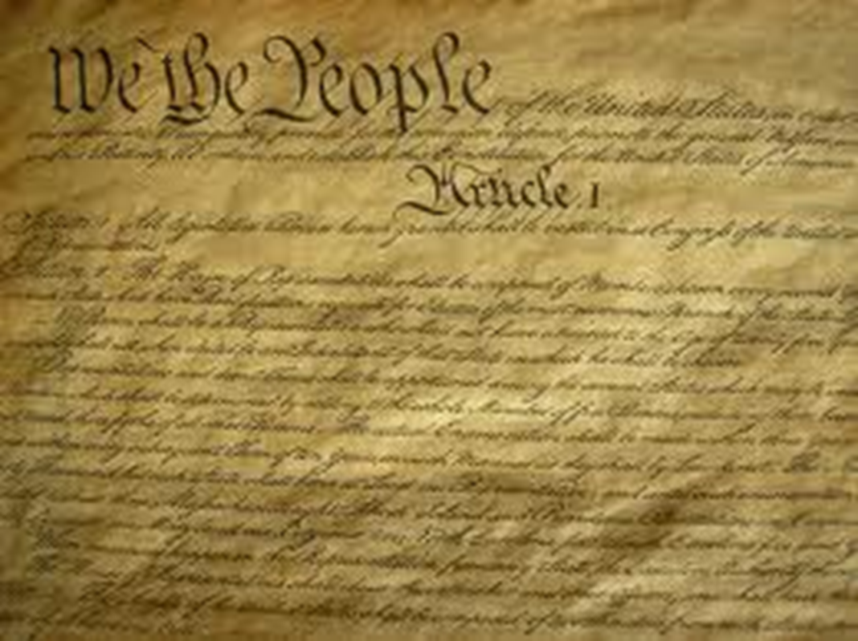
\includegraphics[height=.7\textheight]{img/constitution.png} \\
%   \only<1>{\textbf{Article IV, sec. 3, cl. 2:} ``\ldots nothing in this Constitution shall be so construed as to Prejudice any \emph{claims}\ldots of any particular State.''}
%   \only<2>{\textbf{Article IV, sec. 3, cl. 2:} \st{``\ldots nothing in this Constitution shall be so construed as to Prejudice any \emph{claims}\ldots of any particular State.''}}
%\end{frame}
%
%\begin{frame}{Engagements Clause}
%   \centering
%   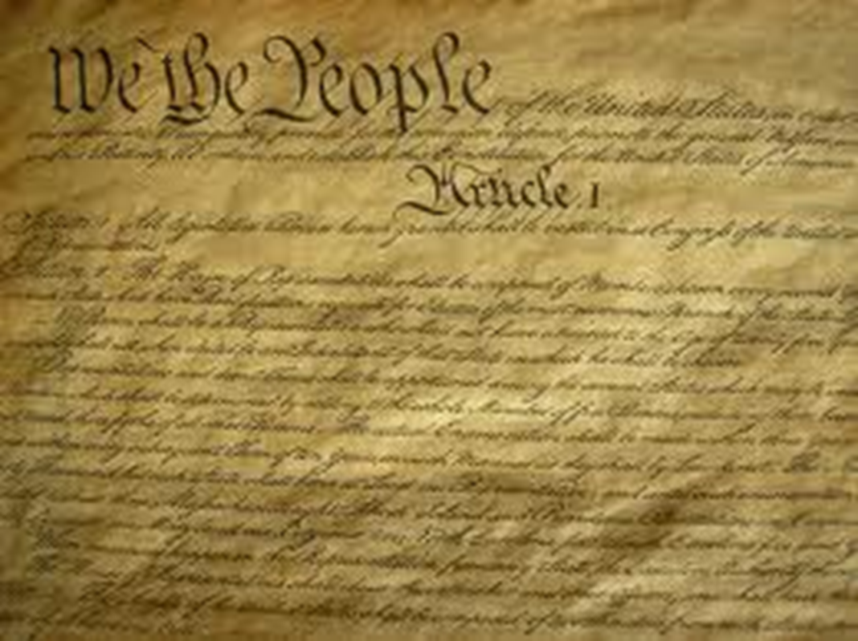
\includegraphics[height=.7\textheight]{img/constitution.png} \\
%   \only<1>{\textbf{Article VI, clause 1:} ``All\ldots \emph{Engagements} entered into,
%   before the Adoption of this Constitution, shall be as valid against the
%   United States under this Constitution, as under the Confederation.''}
%   \only<2>{\textbf{Article VI, clause 1:} \st{``All\ldots \emph{Engagements} entered into,
%   before the Adoption of this Constitution, shall be as valid against the
%   United States under this Constitution, as under the Confederation.''}}
%\end{frame}
%
%\begin{frame}{Engagements Clause}
%   \centering
%   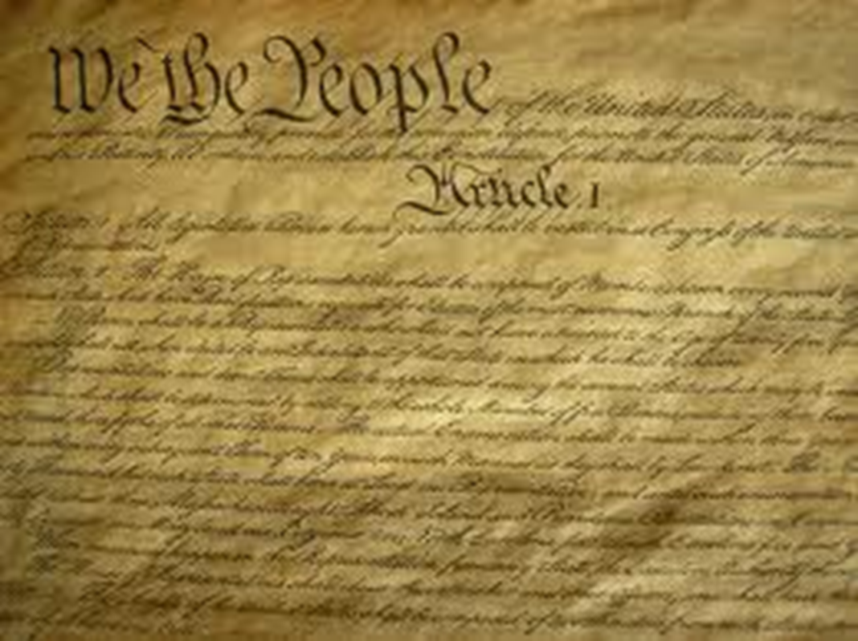
\includegraphics[height=.7\textheight]{img/constitution.png} \\
%   By an act of Congress, the Constitution was amended by a change in policy to
%   abandon the requirement to dispose of territorial and public land.
%\end{frame}
%
%\begin{frame}{Jurisdiction Clause Family}
%    \centering
%    
\includegraphics[height=0.85\textheight]{img/family.png} \\
%    \huge{\textbf{ \color{white}
%        \Put(25, 300){\begin{sideways}\colorbox{blue}{Admissions}\end{sideways}}
%        \Put(60, 300){\begin{sideways}\colorbox{blue}{Claims}\end{sideways}}
%        \Put(90, 300){\begin{sideways}\colorbox{blue}{Property}\end{sideways}}
%        \Put(134, 300){\begin{sideways}\colorbox{blue}{Guarantee}\end{sideways}}
%        \Put(168, 300){\begin{sideways}\colorbox{blue}{Enclave}\end{sideways}}
%        \Put(200, 300){\begin{sideways}\colorbox{blue}{Engagements}\end{sideways}}
%        \Put(235, 300){\begin{sideways}\colorbox{blue}{Supremacy}\end{sideways}}
%    }}
%\end{frame}
%
%\begin{frame}{Jurisdiction Clause Family}
%    \centering
%    
\includegraphics[height=0.85\textheight]{img/family.png} \\
%    \huge{\textbf{ \color{white}
%        \Put(17, 300){ \begin{sideways}\colorbox{red}{\st{Admissions}}\end{sideways}}
%        \Put(52, 300){ \begin{sideways}\colorbox{red}{\st{Claims}}\end{sideways}}
%        \Put(82, 300){ \begin{sideways}\colorbox{red}{\st{Property}}\end{sideways}}
%        \Put(134, 300){\begin{sideways}\colorbox{red}{\st{Guarantee}}\end{sideways}}
%        \Put(168, 300){\begin{sideways}\colorbox{red}{\st{Enclave}}\end{sideways}}
%        \Put(200, 300){\begin{sideways}\colorbox{red}{\st{Engagements}}\end{sideways}}
%        \Put(235, 300){\begin{sideways}\colorbox{red}{\st{Supremacy}}\end{sideways}}
%    }}
%\end{frame}
%
%\begin{frame}
%    \centering
%    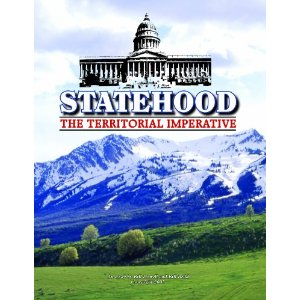
\includegraphics[height=.9\textheight]{img/territorial-imperative} \\
%    Bill Howell, Bill Redd --- 2005, 524 pages \\
%\end{frame}
%
%\begin{frame}{The World's Plan for Happiness}
%    \centering
%    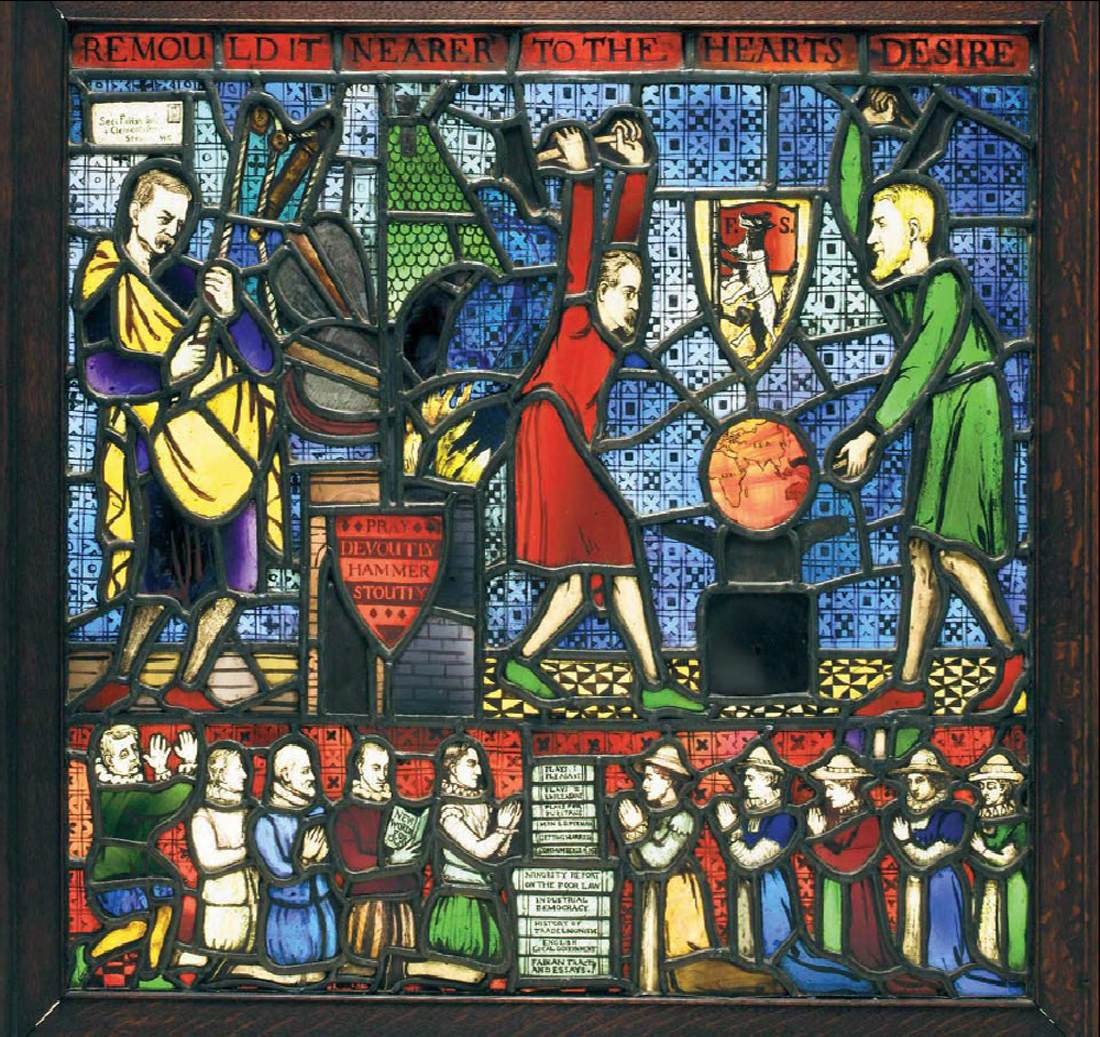
\includegraphics[height=.9\textheight]{img/remold-it.jpg} \\
%\end{frame}
%
%\begin{frame}{Evolutionary Socialism, 1910}
%    \centering
%    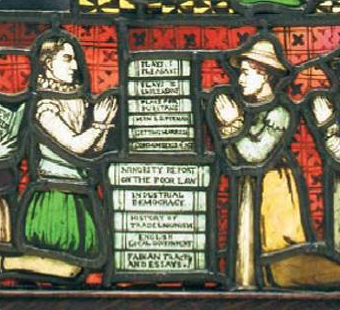
\includegraphics[height=.9\textheight]{img/remold-it-small.png} \\
%\end{frame}
%
%\begin{frame}{Fundamental Principles of Socialism}
%    \centering
%    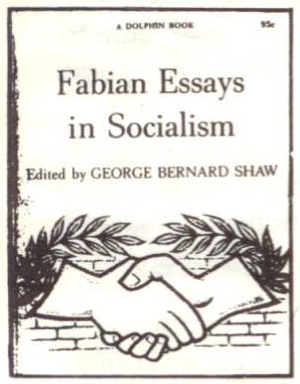
\includegraphics[height=.9\textheight]{img/fabian.png} \\
%\end{frame}
%
%\begin{frame}{Fundamental Principles of Socialism}
%    \centering
%    1. Government ownership \emph{or control} of all land \\
%    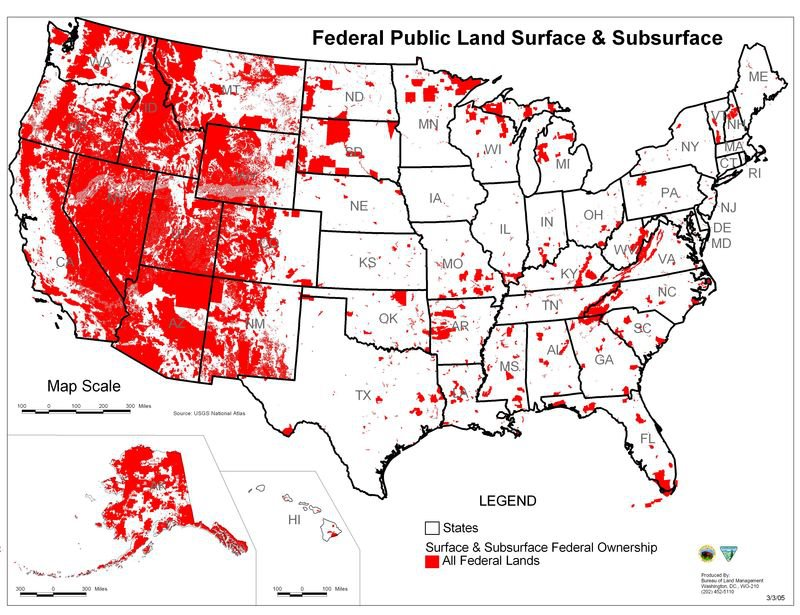
\includegraphics[height=.9\textheight]{img/federal-lands.png} \\
%\end{frame}
%
%\begin{frame}{Government Ownership of Nevada}
%    \centering
%    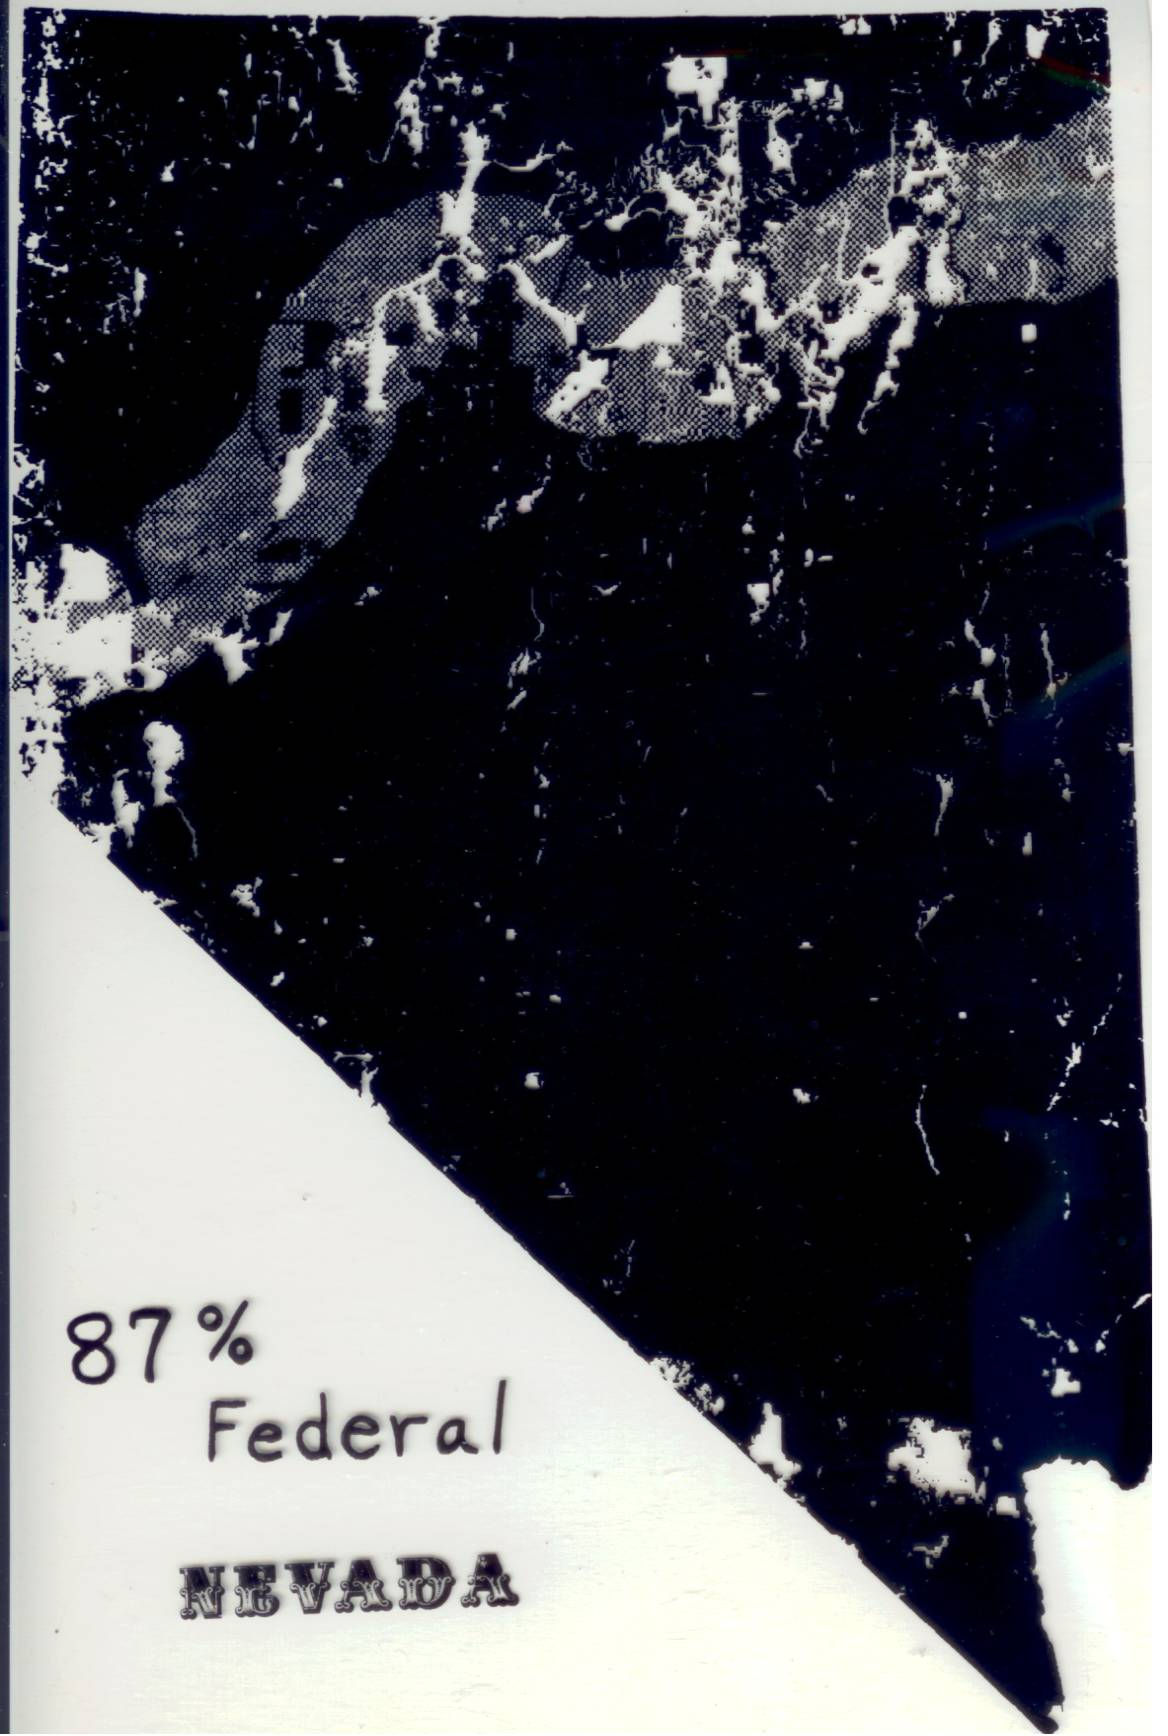
\includegraphics[width=.9\textwidth]{img/nevada.jpg} \\
%\end{frame}
%
%\begin{frame}{Fundamental Principles of Socialism}
%    \centering
%    2. Government ownership \emph{or control} of major industries\\
%    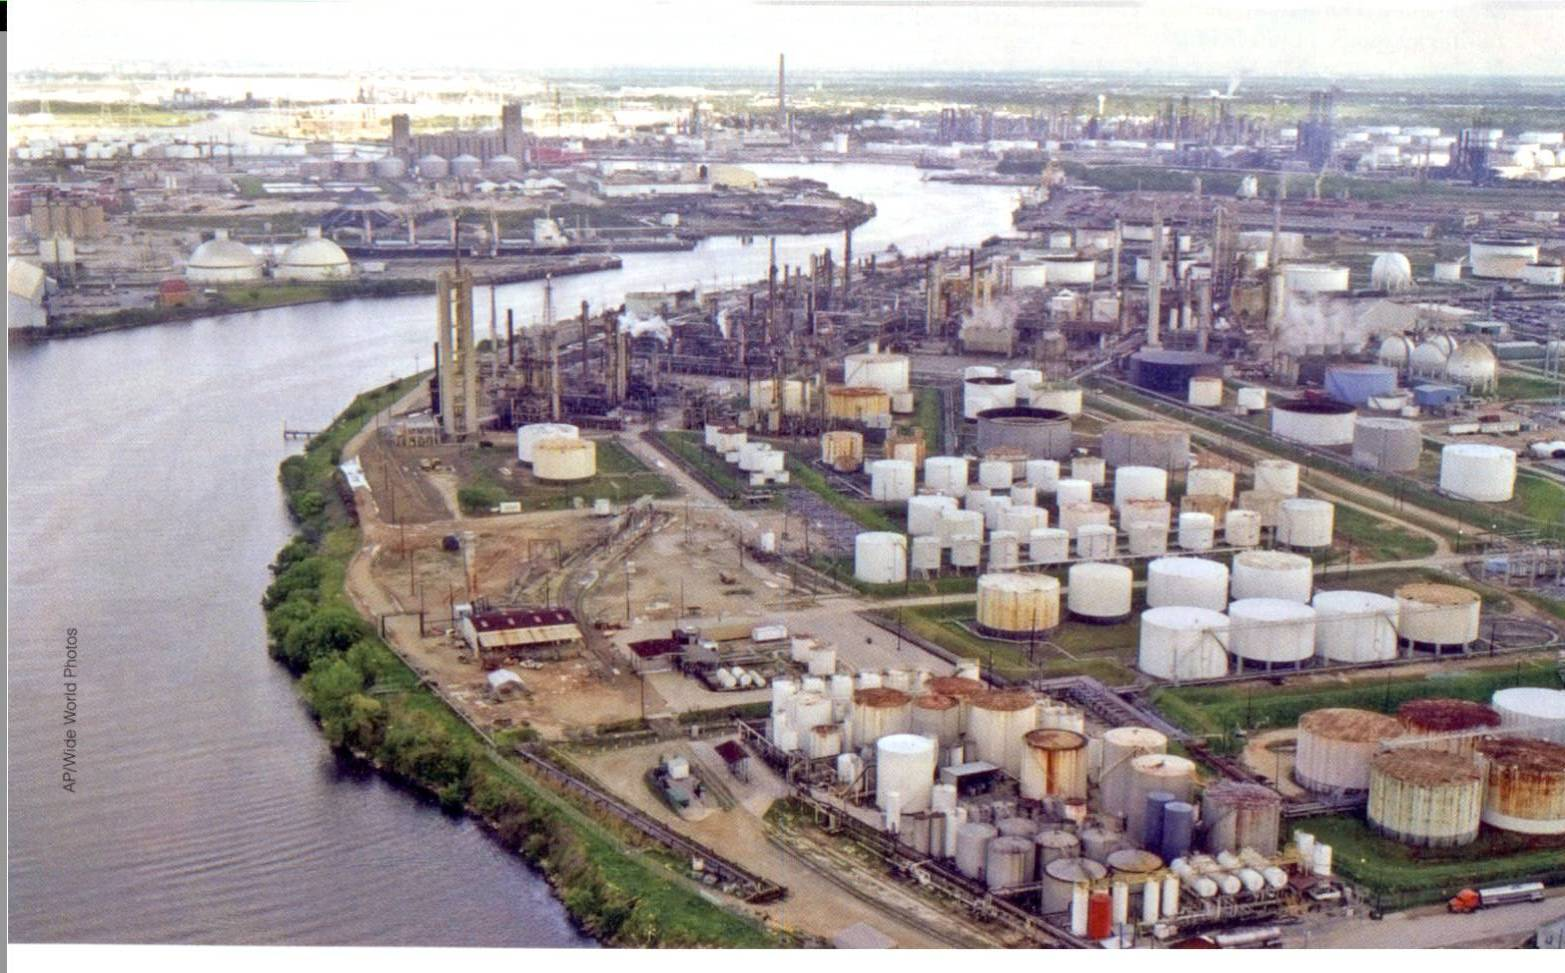
\includegraphics[width=.9\textwidth]{img/industries.jpg} \\
%\end{frame}
%
%\begin{frame}{Fundamental Principles of Socialism}
%    \centering
%    3. Government control over labor \\
%    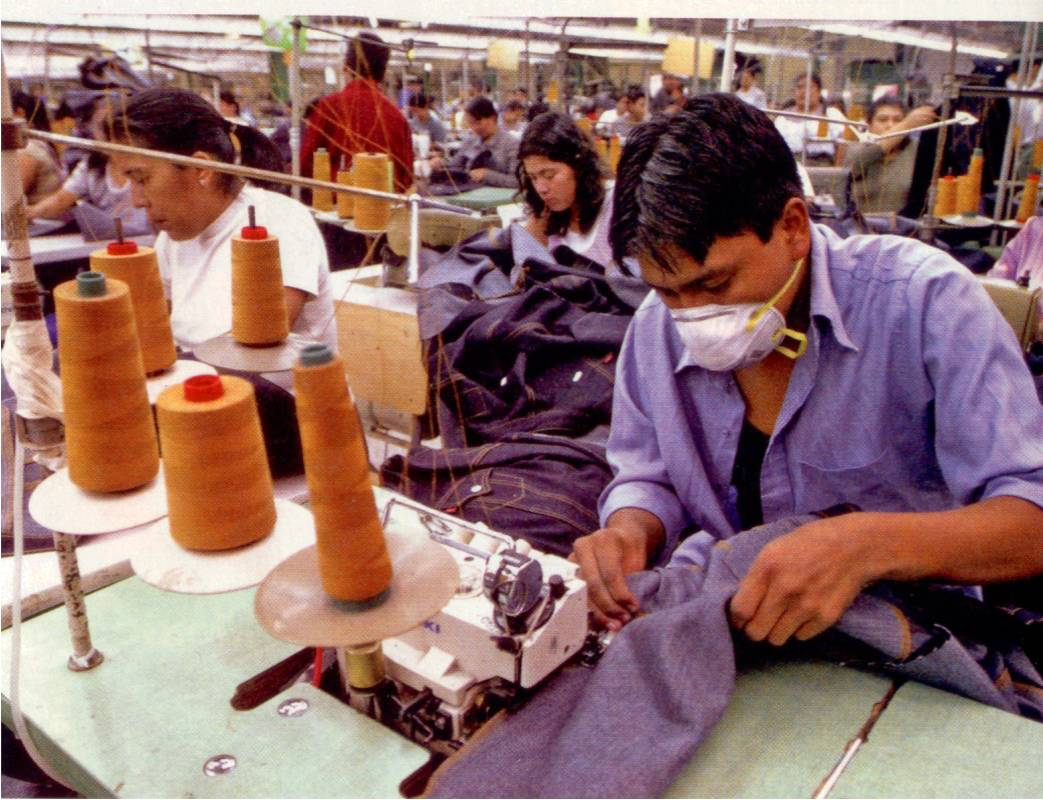
\includegraphics[width=.9\textwidth]{img/labor.jpg} \\
%\end{frame}
%
%\begin{frame}{Fundamental Principles of Socialism}
%    \centering
%    4. Government ownership \emph{or control} of communications and transportation \\
%    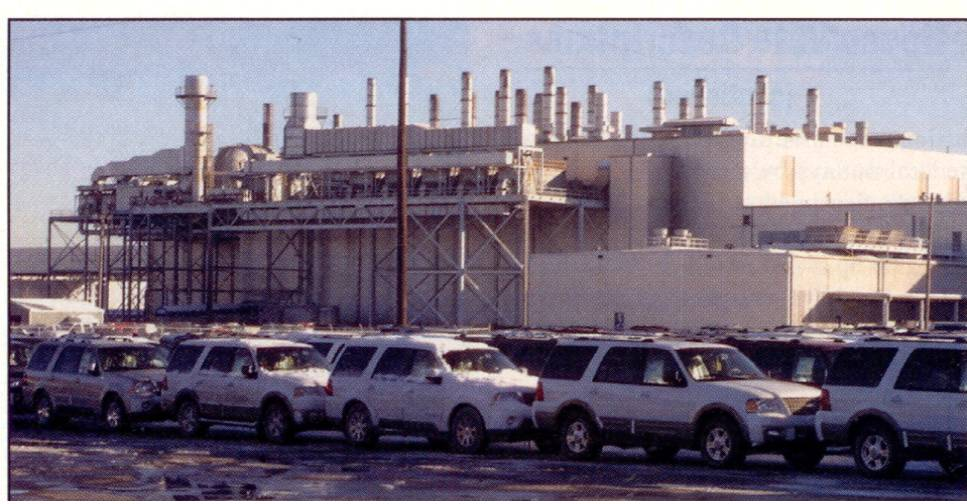
\includegraphics[width=.9\textwidth]{img/transportation.jpg} \\
%\end{frame}
%
%\begin{frame}{Fundamental Principles of Socialism}
%    \centering
%    5. Government control of all credit \\
%    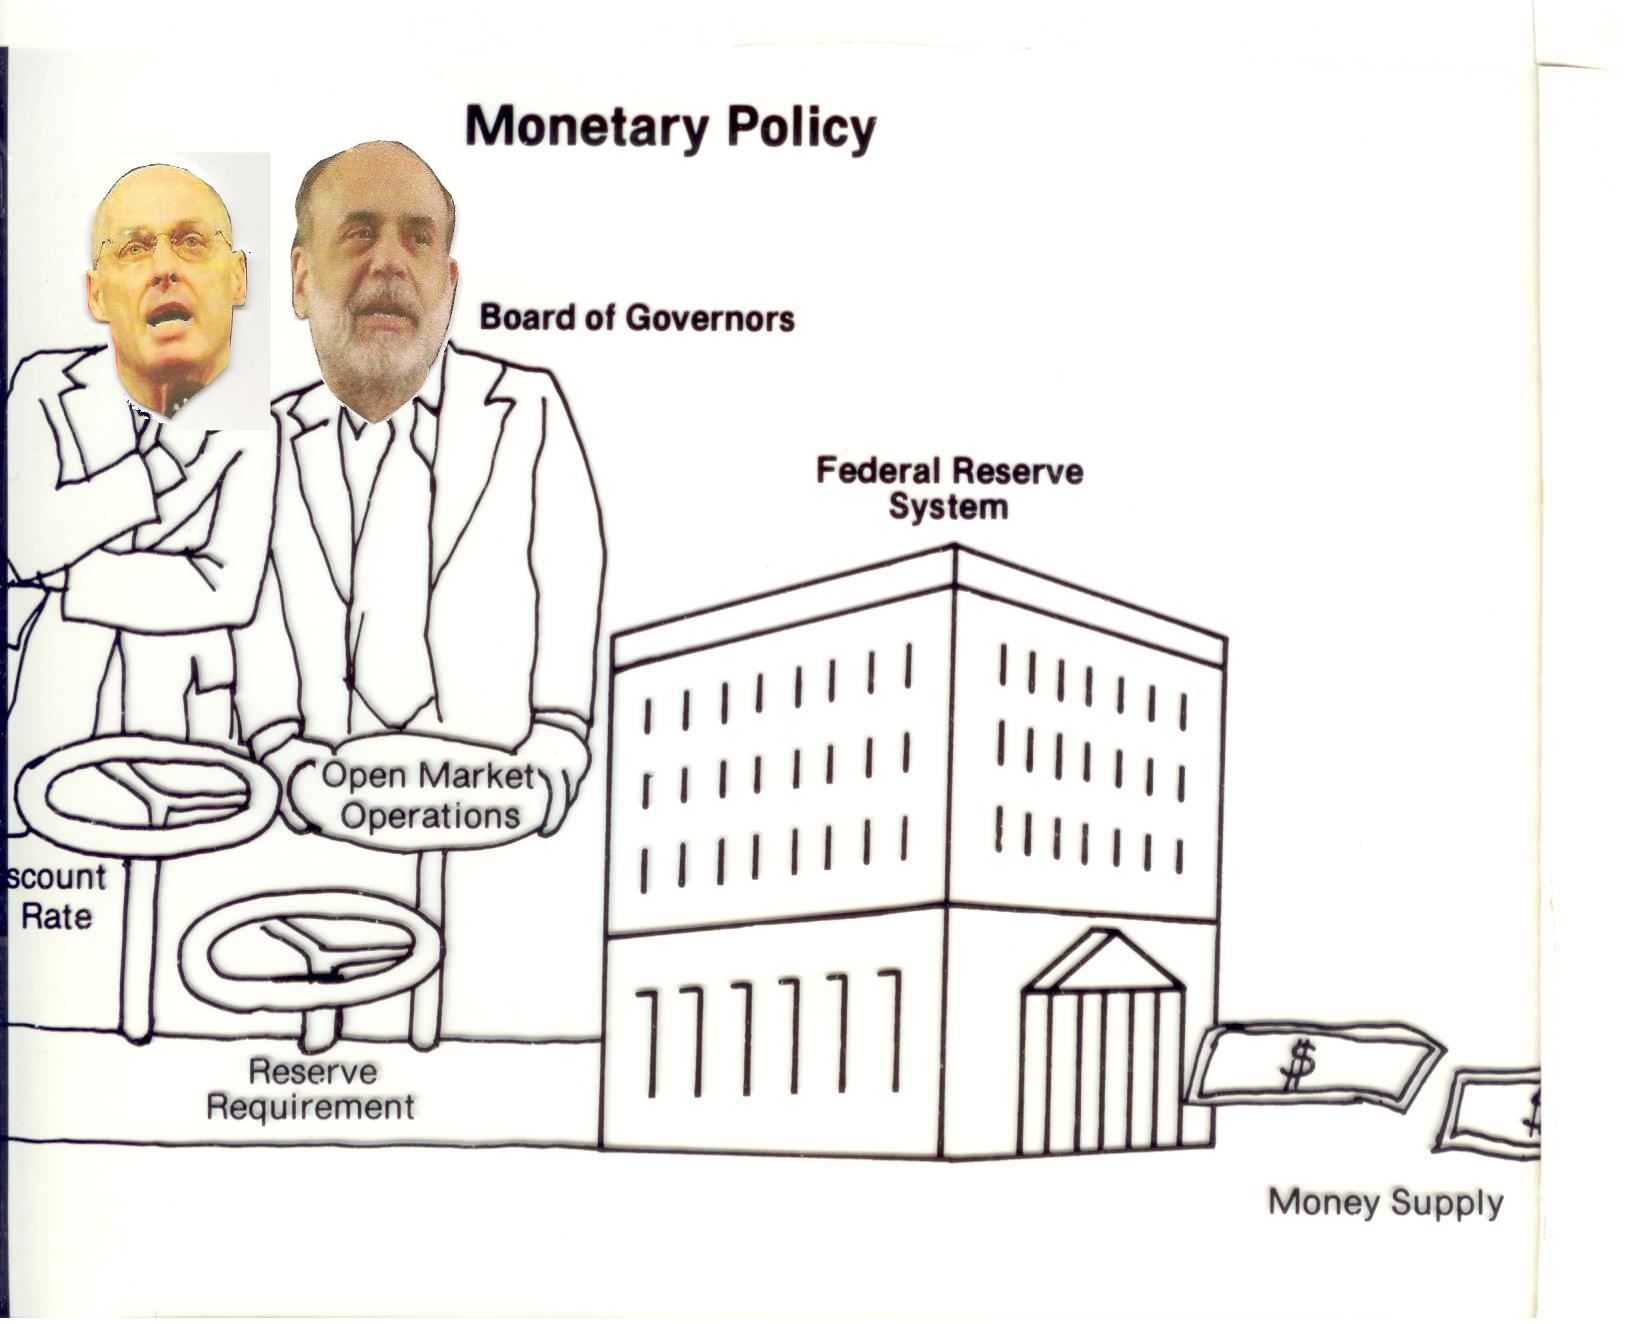
\includegraphics[width=.9\textwidth]{img/credit.png} \\
%\end{frame}
%
%\begin{frame}{Fundamental Principles of Socialism}
%    \centering
%    6. Government control of all insurance \\
%    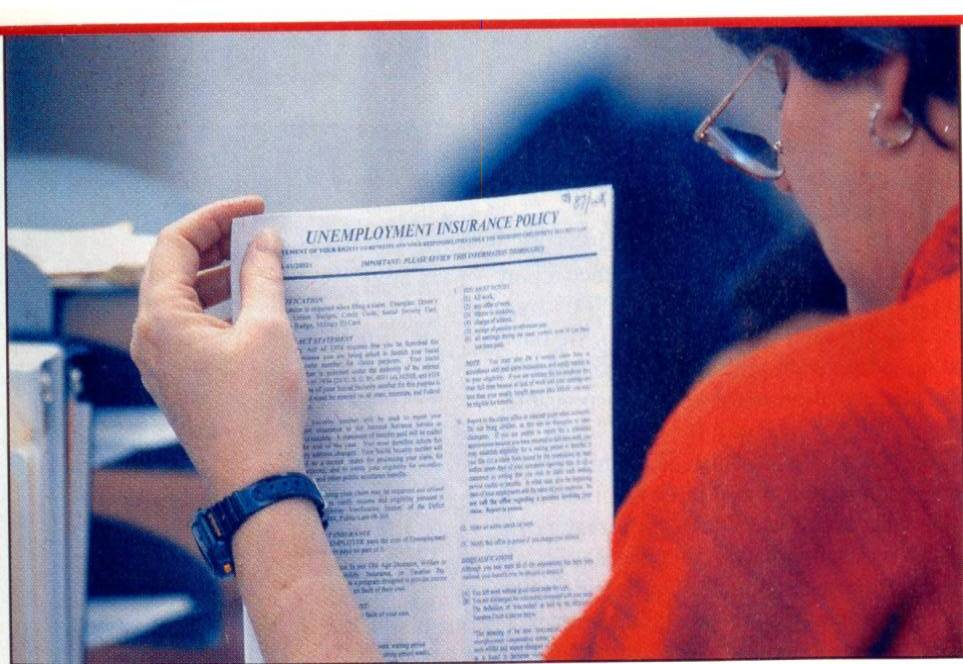
\includegraphics[width=.9\textwidth]{img/insurance.jpg} \\
%\end{frame}
%
%\begin{frame}{Fundamental Principles of Socialism}
%    \centering
%    7. Government control of the educational system \\
%    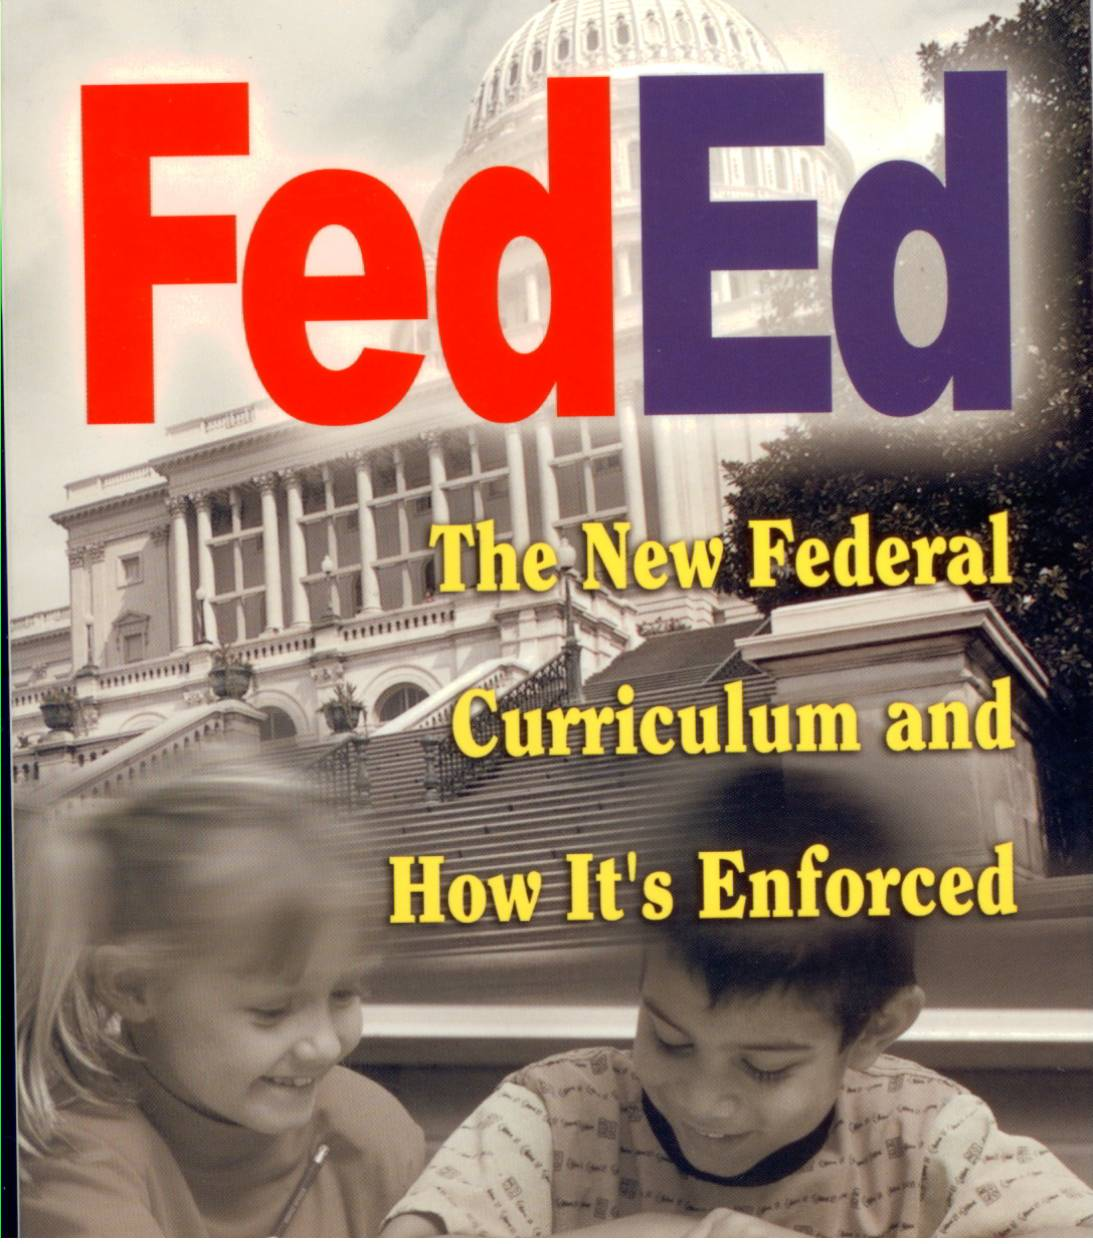
\includegraphics[height=.9\textheight]{img/education.jpg} \\
%\end{frame}
%
%\begin{frame}{Fundamental Principles of Socialism}
%    \centering
%    8. Elimination of the significance of the family \\
%    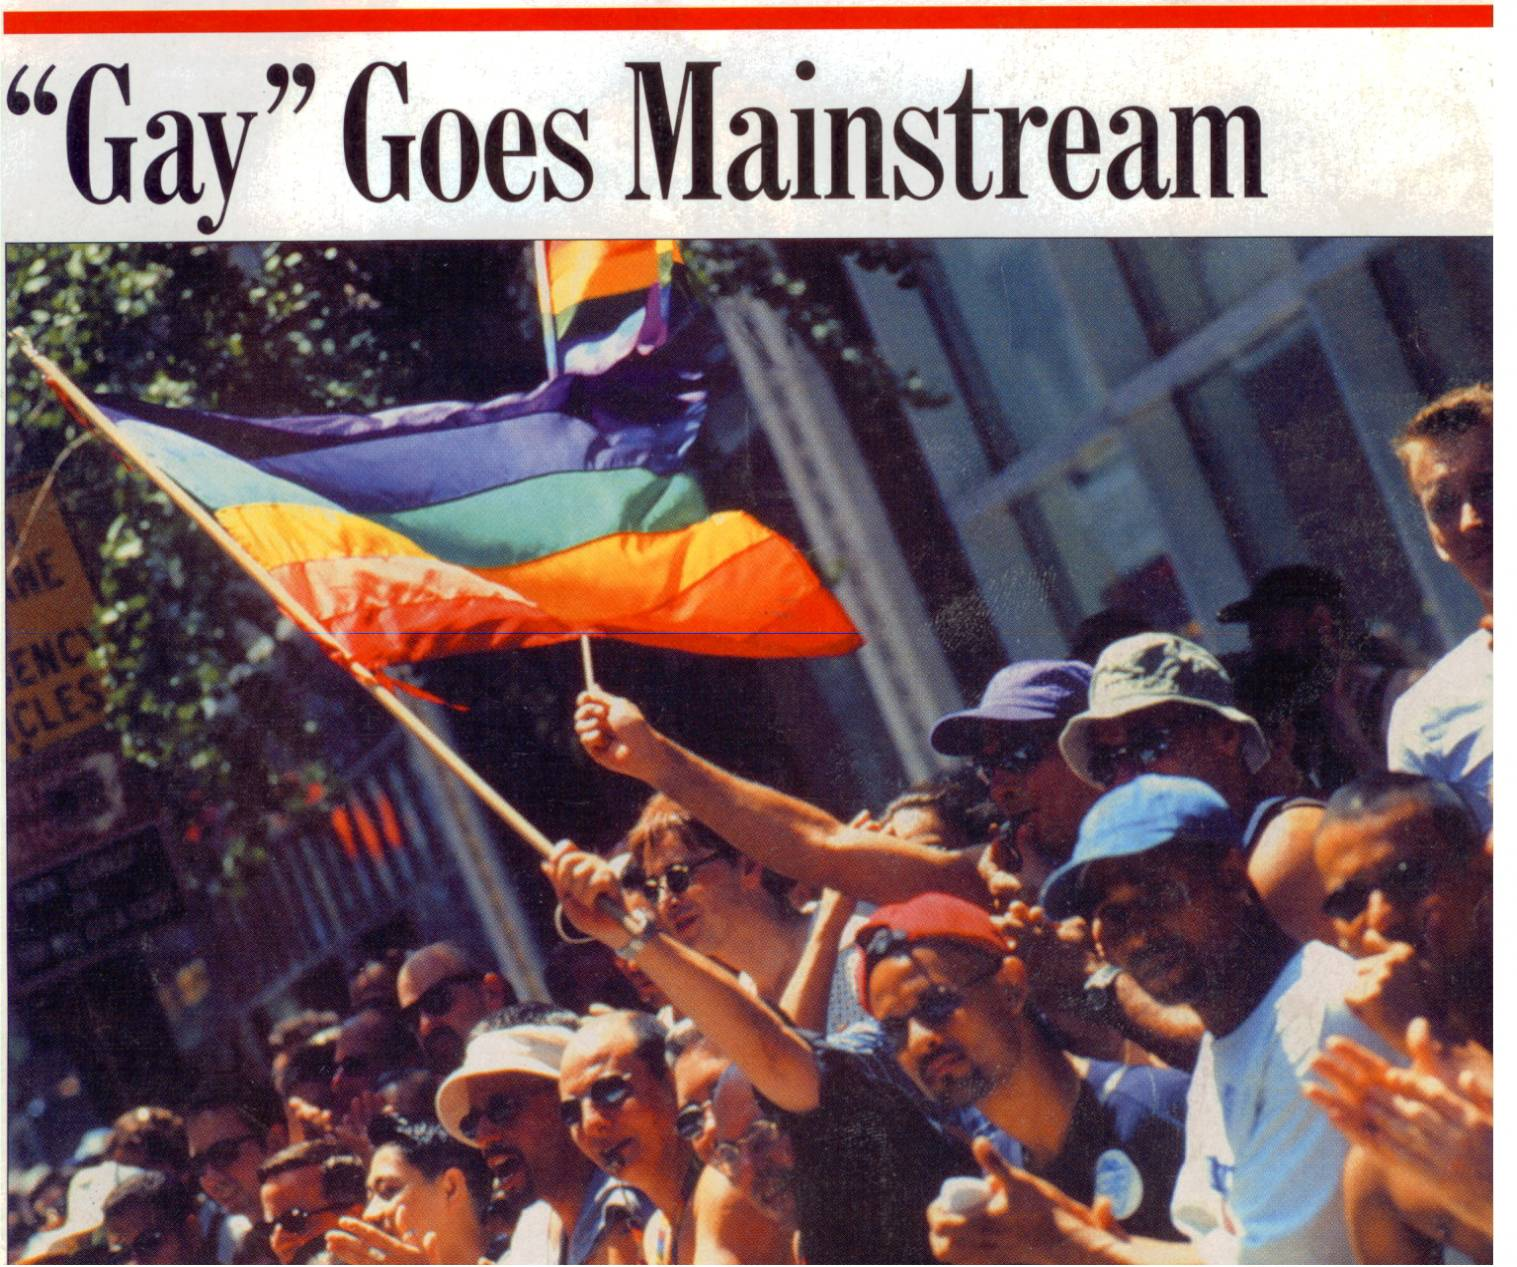
\includegraphics[height=.9\textheight]{img/gay.jpg} \\
%\end{frame}
%
%\begin{frame}{Fundamental Principles of Socialism}
%    \centering
%    9. Elimination of the significance of religion \\
%    \only<1>{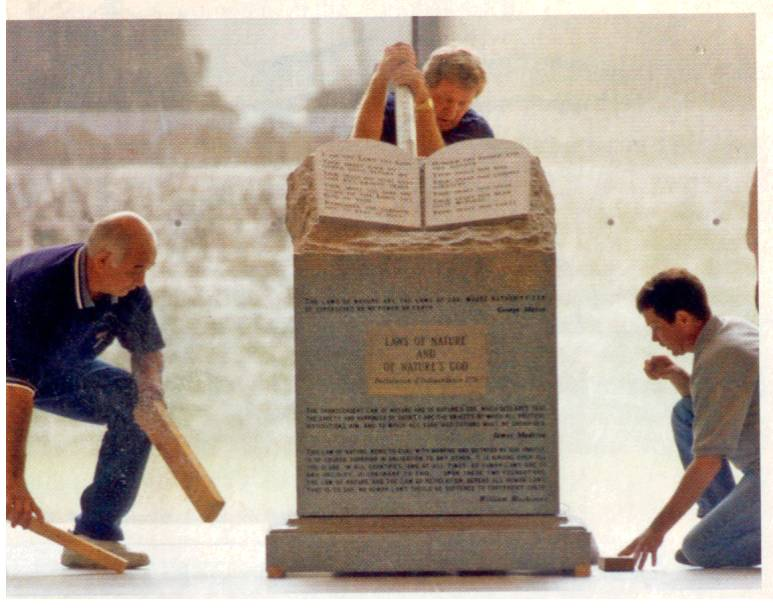
\includegraphics[width=.9\textwidth]{img/10-commandments.jpg} \\}
%    \only<2>{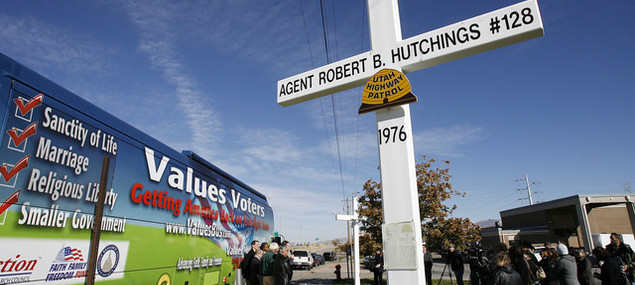
\includegraphics[width=.9\textwidth]{img/religion.png} \\}
%\end{frame}
%
%\begin{frame}{Fundamental Principles of Socialism}
%    \centering
%    10. Establishment of a minimum wage \\
%    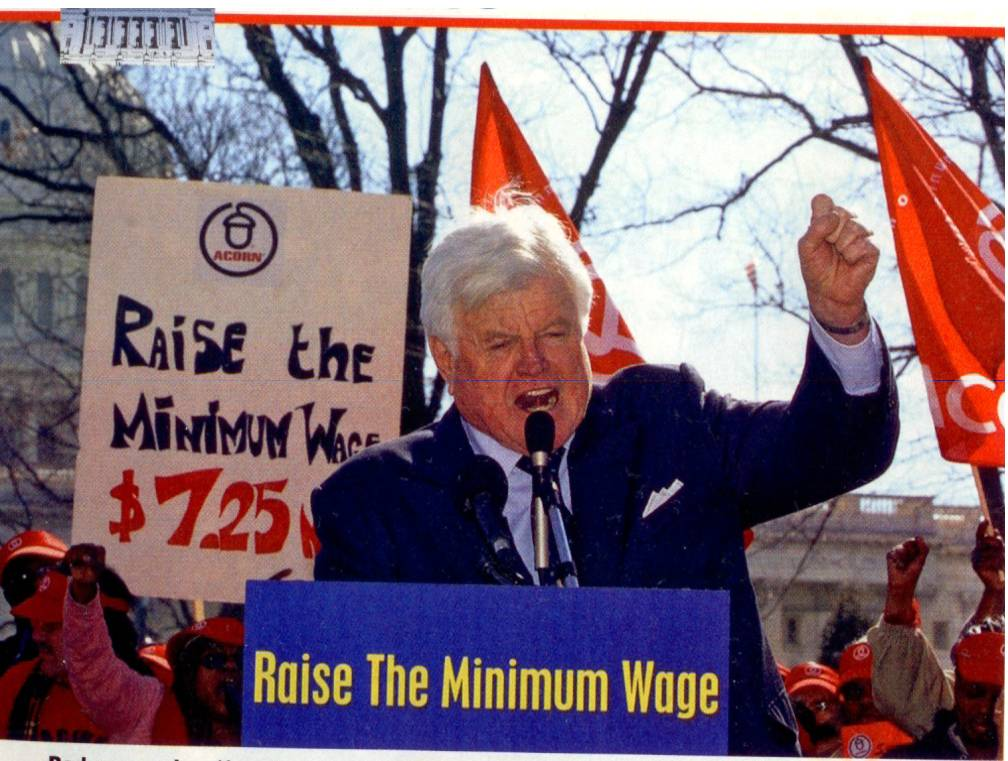
\includegraphics[width=.9\textwidth]{img/wage.jpg} \\
%\end{frame}
%
%\begin{frame}{Fundamental Principles of Socialism}
%    \centering
%    11. A universal system of pensions \\
%    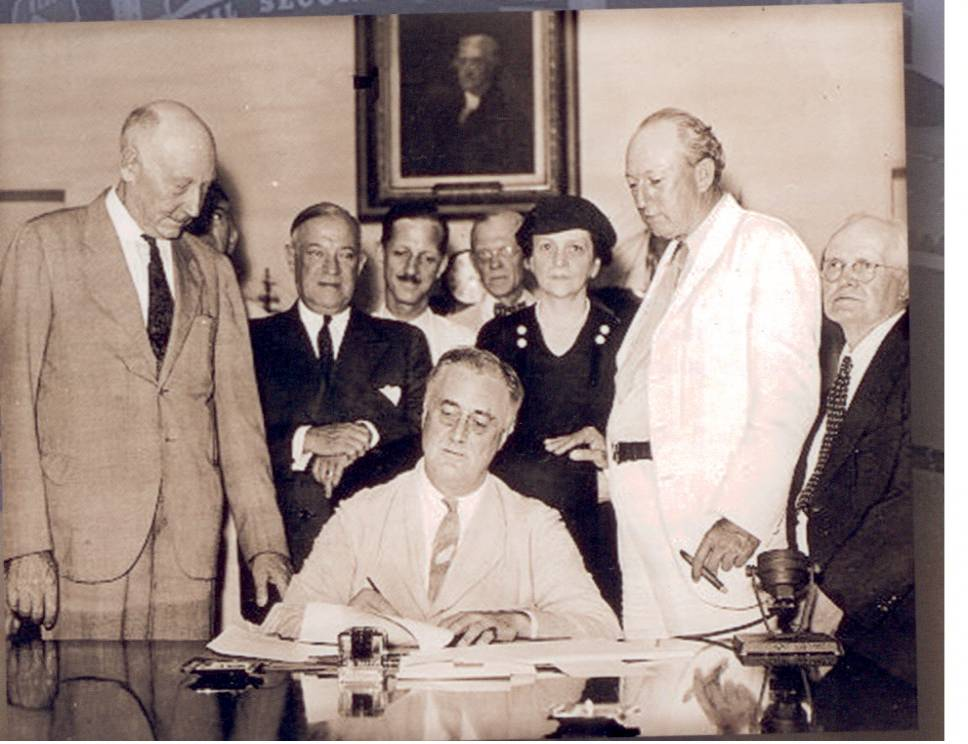
\includegraphics[width=.9\textwidth]{img/pensions.jpg} \\
%\end{frame}
%
%\begin{frame}{Fundamental Principles of Socialism}
%    \centering
%    12. Justified use of force if necessary to attain socialistic goals
%    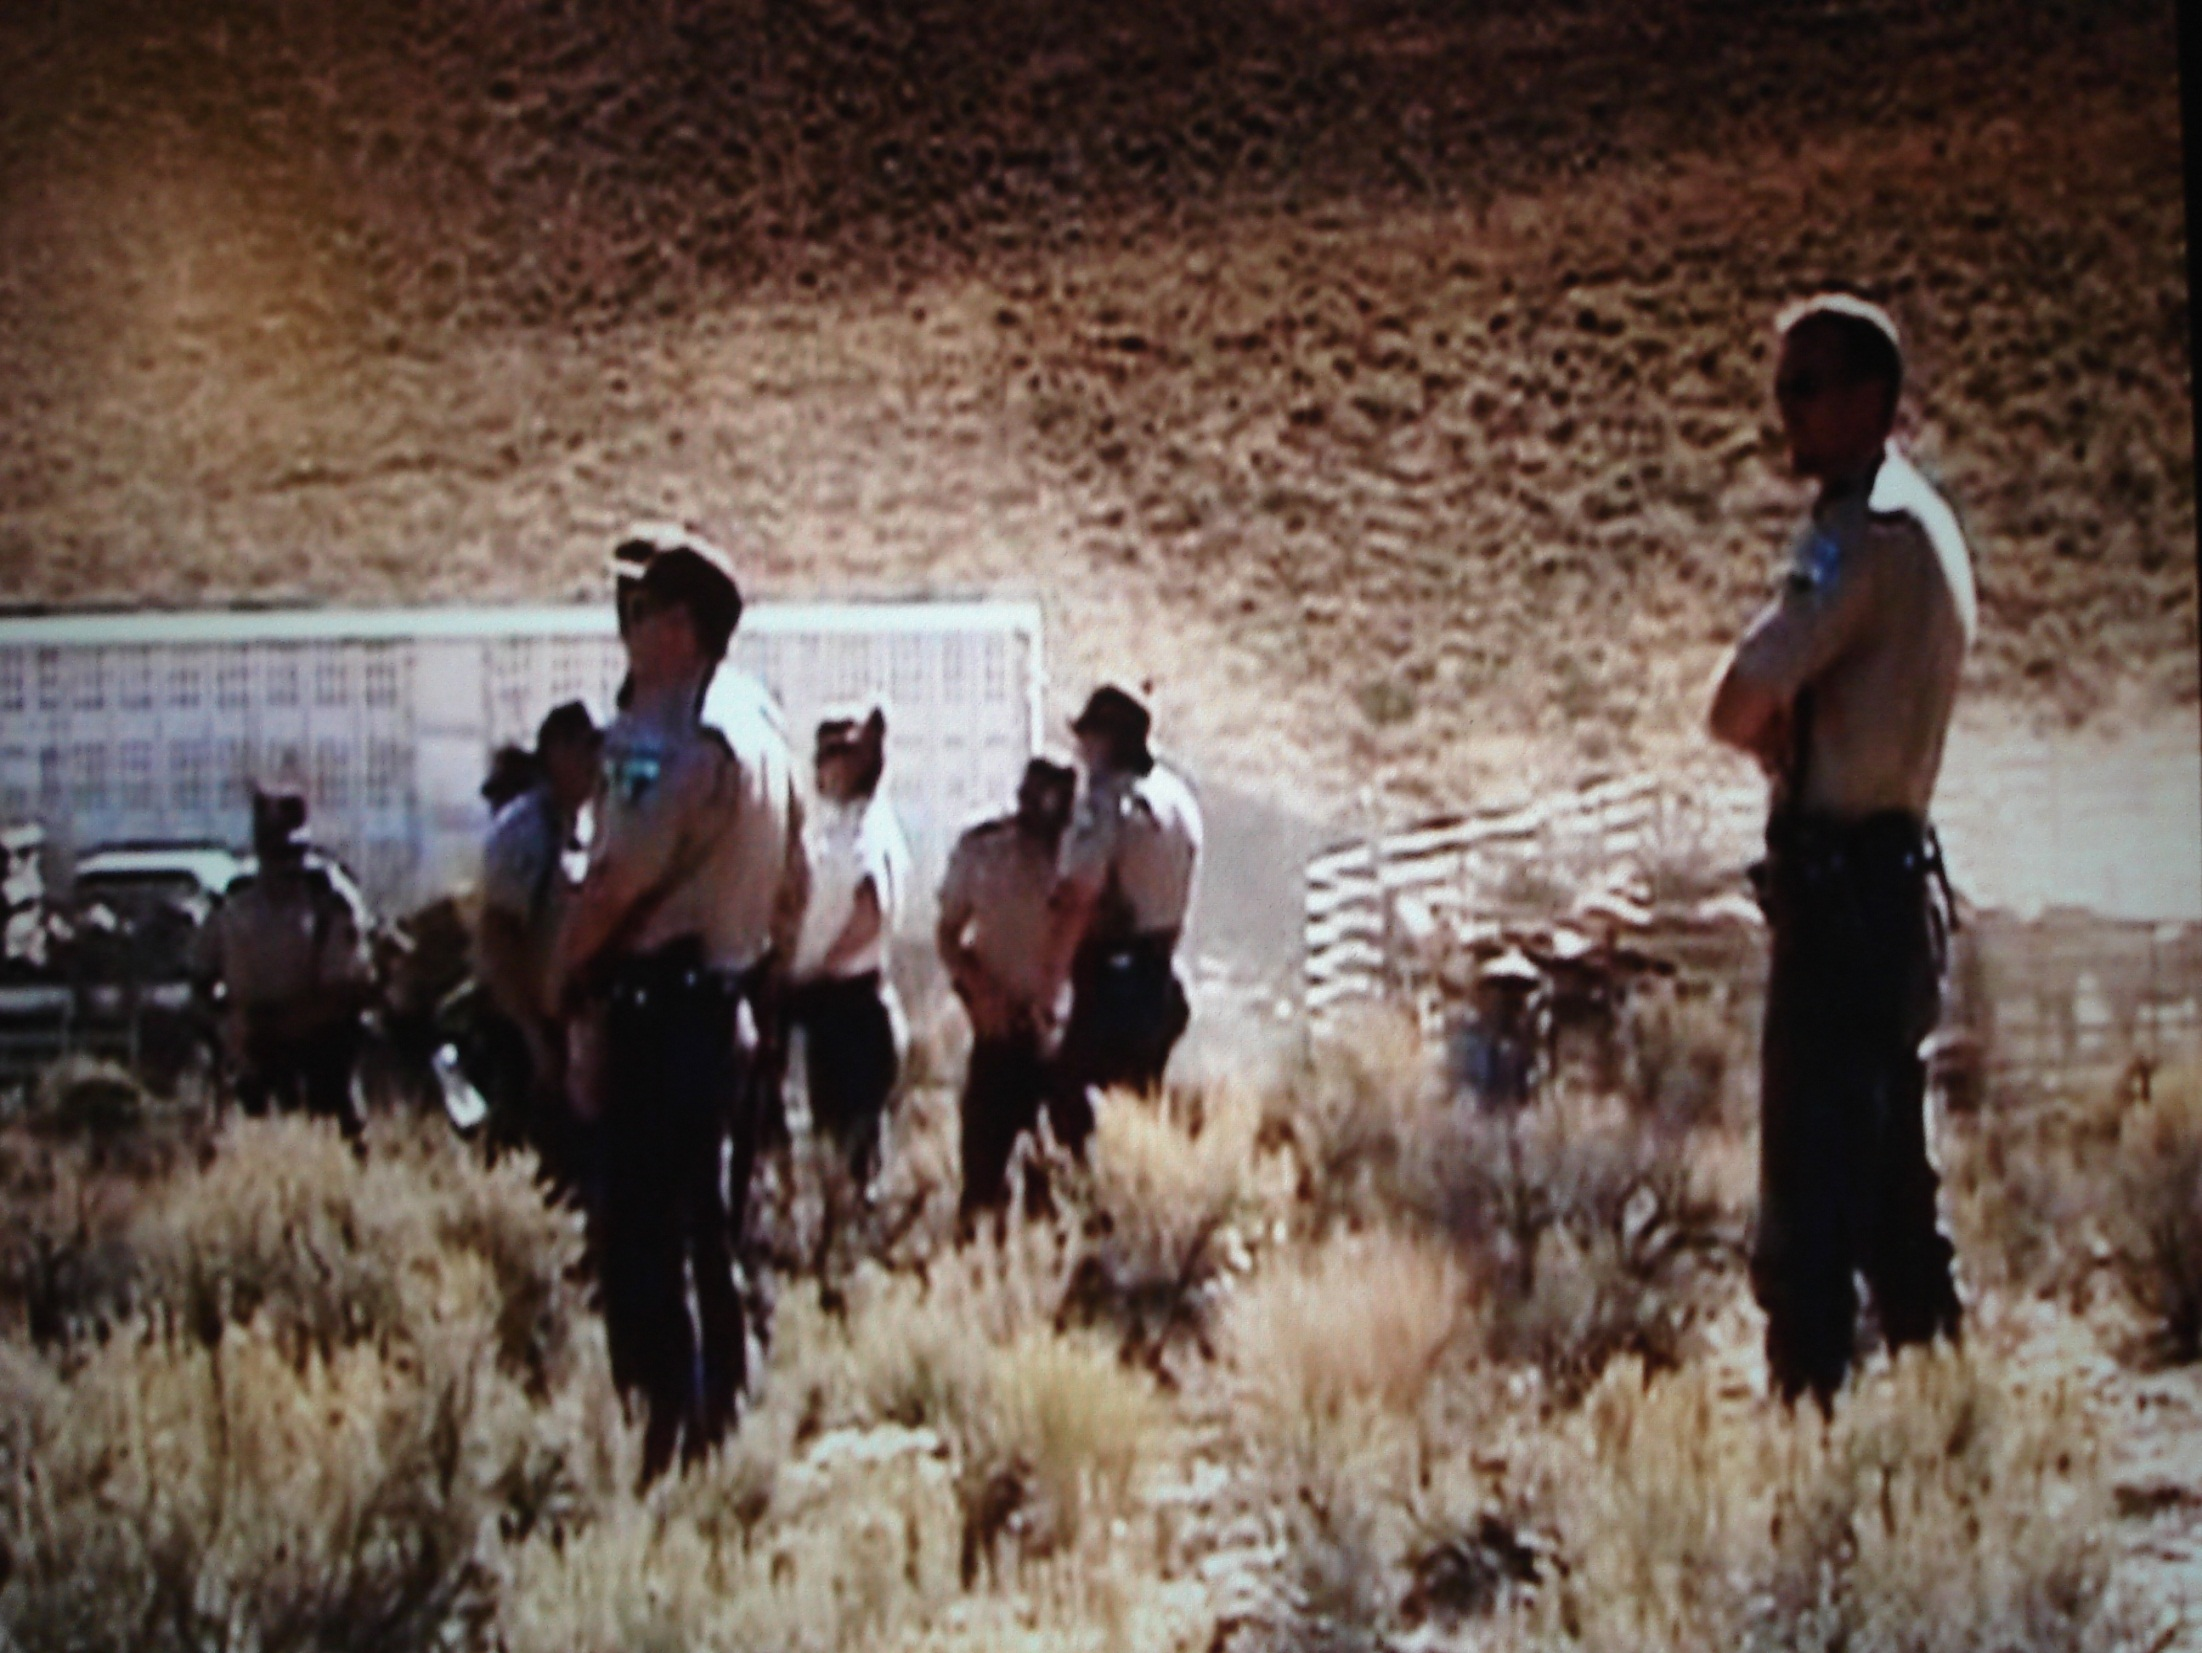
\includegraphics[width=.9\textwidth]{img/justified-force.jpg} \\
%\end{frame}
%
%\begin{frame}{Fundamental Principles of Socialism}
%    \centering
%    13. Graduated income tax \\
%    \includegraphics[width=.9\textwidth]{img/graduated-tax.jpg} \\
%    \only<2>{``Tell us where you are, and we'll send you money!''}
%\end{frame}
%
%\begin{frame}{Fundamental Principles of Socialism}
%    \begin{enumerate}
%        \item Government ownership or control of all land
%        \item Government ownership or control of major industries
%        \item Government control over labor
%        \item Government ownership or control of communications and transportation
%        \item Government control of all credit
%        \item Government control of all insurance
%        \item Government control of the educational system
%        \item Elimination of the significance of the family
%        \item Elimination of the significance of religion
%        \item Establishment of a minimum wage
%        \item A universal system of pensions
%        \item Justified use of force where necessary to attain socialistic goals
%        \item Graduated income tax
%    \end{enumerate}
%\end{frame}
%
%\begin{frame}{1910}
%    \begin{columns}[onlytextwidth]
%        \column{0.5\textwidth}
%            \centering
%            \includegraphics[width=0.95\textwidth]{img/remold-hammers.png} \\
%            \only<1>{ \color{white} \huge ``Gradual, silent encroachment'' }
%            \only<2>{ \huge ``Gradual, silent encroachment'' }
%
%        \column{0.5\textwidth}
%            \centering
%            \includegraphics[width=0.95\textwidth]{img/wolf.png} \\
%    \end{columns}
%\end{frame}
%
%\begin{frame}{Gradual Encroachment}
%    \centering
%    \includegraphics[width=0.65\textwidth]{img/french-pres.png} \\
%    Val\'{e}ry Giscard d'Estaing \\
%\end{frame}
%
%\begin{frame}{Sustainable Development}
%    \begin{columns}[onlytextwidth]
%        \column{0.5\textwidth}
%            \centering
%            \includegraphics[width=.75\textwidth]{img/agenda-21.png} \\
%
%        \column{0.5\textwidth}
%            \centering
%            \includegraphics[width=.75\textwidth]{img/ghwbush.png} \\
%            President George H. W. Bush, 1992 \\
%    \end{columns}
%\end{frame}
%
%\begin{frame}{U.N. Biodiversity Treaty}
%    \centering
%    \includegraphics[width=0.85\textwidth]{img/biodiversity.png} \\
%    Never ratified by the U.S. Senate \\
%\end{frame}
%
%\begin{frame}{President's Council on Sustainable Development}
%    \begin{columns}[onlytextwidth]
%        \column{0.5\textwidth}
%            \centering
%            \includegraphics[width=.75\textwidth]{img/clinton.png} \\
%            President Bill Clinton \\
%
%        \column{0.5\textwidth}
%            ``We will implement Agenda 21 by administrative laws and executive orders.''
%    \end{columns}
%\end{frame}
%
%\begin{frame}{Antiquities Act, 1906}
%    \begin{columns}[onlytextwidth]
%        \column{0.5\textwidth}
%            \centering
%            Congress has not acted quickly enough to protect federal lands. \\
%            \vspace{20pt}
%            { \Large{``Monument Power'' 22x}}
%
%        \column{0.5\textwidth}
%            \centering
%            \includegraphics[width=.75\textwidth]{img/clinton.png} \\
%            President Bill Clinton \\
%
%    \end{columns}
%\end{frame}
%
%\begin{frame}
%    \centering
%    \includegraphics[width=0.75\textwidth]{img/salazar.png} \\
%    January 10, 2010: Dept. of Interior Secretary Ken Salazar announces
%    \textbf{new mining near the Grand Canyon will be banned on a million acres} \\
%\end{frame}
%
%\begin{frame}{National Monuments}
%    \centering
%    \includegraphics[width=0.75\textwidth]{img/monuments.png} \\
%    \begin{itemize}
%        \item Prohibit natural resource development: timber, mining, oil, natural gas, etc.
%        \item Close roads
%        \item Establish wilderness areas
%        \item Remove dams
%    \end{itemize}
%\end{frame}
%
%\begin{frame}{Yreka, California --- October 22, 2011}
%    \centering
%    \includegraphics[width=0.95\textwidth]{img/yreka.png} \\
%    \vspace{20pt}
%    \only<1>{
%    The Federal Government pays environmental groups to sue the Federal
%    Government to stop the use of your property! For example, \$36 million was
%    paid to 19 environmental groups in 9 years in 19 states. \\
%	Karen-Budd Falen, Property Rights Lawyer \\ }
%    \only<2>{ ``I had spent a good part of my life enforcing the penal code,
%    but not understanding my oath of office.'' \\ Sheriff Dean Wilson \\ }
%    \only<3>{ ``A giant has been awakened, and [the federal bureaucracy] didn't count on that.'' \\
%    Sheriff Greg Hagwood \\ }
%\end{frame}
%
%\begin{frame}{Sheriff Glenn Palmer}
%    \begin{columns}[onlytextwidth]
%        \column{0.5\textwidth}
%            \centering
%            \includegraphics[width=0.75\textwidth]{img/glenn-palmer-letter.png}
%            \\ { \tiny March 31, 2011 }
%        \column{0.5\textwidth}
%            \centering
%            \includegraphics[width=0.75\textwidth]{img/glenn-palmer.png}
%            \\ Sheriff Glenn Palmer
%            \\ Grant County, Oregon
%    \end{columns}
%\end{frame}
%
%\begin{frame}{Sheriff Glenn Palmer}
%    \begin{columns}[onlytextwidth]
%        \column{0.5\textwidth}
%            \centering
%            Where does the United States Forest Service get its Constitutional authority to have law enforcement officers in Grant County?
%        \column{0.5\textwidth}
%            \centering
%            \includegraphics[width=0.75\textwidth]{img/glenn-palmer.png}
%            \\ Sheriff Glenn Palmer
%            \\ Grant County, Oregon
%    \end{columns}
%\end{frame}

\begin{frame}{Sheriff Glenn Palmer}
    \begin{columns}[onlytextwidth]
        \column{0.5\textwidth}
            \centering
            \includegraphics[width=0.75\textwidth]{img/glenn-palmer.png}
            \\ Sheriff Glenn Palmer
            \\ Grant County, Oregon

        \column{0.5\textwidth}
            ``One response that I have received in writing is that their
            authority is given through the Cooperative Policing Agreement that
            this agency has signed in the past. Upon asking for clarification
            and a second request, the response was that I needed to check with
            my District Attorney. Neither response in my opinion is adequate.''
    \end{columns}
\end{frame}

\begin{frame}{USDA, December 20, 2010}
    \begin{columns}[onlytextwidth]
        \column{0.5\textwidth}
            \centering
            \includegraphics[width=0.75\textwidth]{img/usda-letter.png} \\

        \column{0.5\textwidth}
            5301 -- Forest Service \textbf{law enforcement authority} \\
            5301.1 -- Laws
            \indent 1. The Act of June 4, 1897 \\
            \indent 8. The Act of 2004 \\
            \indent 1. Title 7 U.S.C \\
    \end{columns}
\end{frame}

\begin{frame}{Sheriff Glenn Palmer}
    \begin{columns}[onlytextwidth]
        \column{0.5\textwidth}
            \centering
            \includegraphics[width=0.75\textwidth]{img/glenn-palmer.png}
            \\ Sheriff Glenn Palmer
            \\ Grant County, Oregon

        \column{0.5\textwidth}
            { \Large
                ``Constitutional authority,'' \textbf{NOT} ``Law enforcement authority''
                \pause
                Shouldn't their ``constitutional authority'' be referenced to the Constitution?
            }
    \end{columns}
\end{frame}

\begin{frame}
    \centering
    { \Large
        LEGAL UPDATE FOR LAW ENFORCEMENT \\
        NEW MEXICO SHERIFFS' \& POLICE ASSOCIATION \\
        NOVEMBER 10, 2011 \\
        ********* \\
        FOREST SERVICE LAW ENFORCEMENT AUTHORITIES \\
        \vspace{20pt}
        Prepared by:
        Kenneth D. Paur, Assistant Regional Attorney \\
        U.S.D.A. Office of the General Counsel \\
        Ogden, Utah \\
        (801) 625-5440 kenneth.paur@oge.usda.gov \\
        (Twenty pages) \\
    }
\end{frame}

\begin{frame}{Legal Update for Law Enforcement, New Mexico}
    \begin{varblock}[.9\textwidth]{}
        ``Property Clause''\ldots
        ``Property Clause''\ldots
        ``Property Clause''\ldots
        Supreme Court rejected the need for State consent\ldots
        Supreme Court rejected\ldots
        ``Supremacy Clause''\ldots
    \end{varblock}
\end{frame}

\begin{frame}{Legal Update for Law Enforcement, New Mexico}
    \begin{varblock}[.9\textwidth]{Page 3}
        ``The federal enabling statute imposed several conditions for
        recognition of a state and admission into the Union, including the
        requirement that \textbf{\emph{the state and its citizens forever
        disclaim any right or title to the federal lands within the state}}.''
    \end{varblock}
\end{frame}

\begin{frame}{Legal Update for Law Enforcement, New Mexico}
    \begin{varblock}[.9\textwidth]{Page 20}
        ``Tens of thousands of criminal cases have been investigated and
        prosecuted, and convictions obtained for violation of laws relating to
        the national forests during this time [from 1891 to 2011].''
    \end{varblock}
\end{frame}

\begin{frame}{Sheriff Gil Gilbertson}
    \begin{columns}[onlytextwidth]
        \column{0.5\textwidth}
            \centering
            Where does the United States Forest Service's authority come from?
            \\ { \tiny October, 2011 }
        \column{0.5\textwidth}
            \centering
            \includegraphics[width=0.75\textwidth]{img/gil-gilbertson.png}
            \\ Sheriff Gil Gilbertson
            \\ Josephine County, Oregon
    \end{columns}
\end{frame}

\begin{frame}{James Madison}
    \begin{columns}[onlytextwidth]
        \column{0.5\textwidth}
            \centering
            \includegraphics[width=0.75\textwidth]{img/madison.jpg} \\
        \column{0.5\textwidth}
            ``Since the general civilization of mankind, I believe there are more instances of the abridgment of the freedom of the people by \emph{gradual and silent encroachments} of those in power, than by violent and sudden usurpation.''
    \end{columns}
\end{frame}

\begin{frame}{Sheriff Gil Gilbertson}
    \begin{columns}[onlytextwidth]
        \column{0.5\textwidth}
            \centering
            Where does the United States Forest Service's authority come from? \\
            \vspace{20pt}
            \textbf{ \Large \color{red}
                From ``gradual and silent encroachments''
            }
        \column{0.5\textwidth}
            \centering
            \includegraphics[width=0.75\textwidth]{img/gil-gilbertson.png}
            \\ Sheriff Gil Gilbertson
            \\ Josephine County, Oregon
    \end{columns}
\end{frame}

\begin{frame}{The Truth Is:}
    \large
    The U.S. Forest Service and BLM have NO \textbf{Constitutional authority}.
    By judicial misconstruction of the Property clause, social do-gooders have
    reinvented the structure of the United States' government.
\end{frame}

\begin{frame}{Utah Governor's Race, 2012}
    \centering
    \includegraphics[width=0.8\textwidth,height=.5\textwidth,keepaspectratio=true]{img/gov.png} \\
    { \Large These three candidates for Utah governor said they would \emph{actively fight to regain state control of federal land} in Utah, refuse federal funding, and apply ``nullification.'' (Jan, 2012) \\ }
\end{frame}

\begin{frame}{What is this?}
    \centering
    \includegraphics[height=0.95\textheight]{img/rack.png} \\
\end{frame}

\begin{frame}
    \begin{minipage}{0.2\textwidth}
        \centering
        \only<1,2>{\includegraphics[width=0.9\textwidth]{img/white-wolf.png} \\}
        \only<4->{\includegraphics[width=0.9\textwidth]{img/wolf.png} \\}
        \only<1-4>{\includegraphics[width=0.9\textwidth]{img/white-wolf.png} \\}
        \only<5->{\includegraphics[width=0.9\textwidth]{img/turtle.png} \\}
    \end{minipage}
    \begin{minipage}{0.5\textwidth}
        \centering
        \includegraphics[height=0.9\textheight]{img/rack.png}
        \only<6->{\Put(-120,210){\includegraphics[width=.6\textwidth]{img/us-map-stretched.png}}}
    \end{minipage}
    \begin{minipage}{0.2\textwidth}
        \centering
        \only<2->{\includegraphics[width=0.9\textwidth]{img/national-seal.png} \\ }
        \only<3->{\includegraphics[height=0.5\textheight]{img/fasces.png}}
    \end{minipage}
\end{frame}

\end{document}
